%

% Used for displaying a sample figure. If possible, figure files should
% be included in EPS format.
%
% If you use the hyperref package, please uncomment the following line
% to display URLs in blue roman font according to Springer's eBook style:
% \renewcommand\UrlFont{\color{blue}\rmfamily}
%
%\lstset{language=scafi}
% Please use the
%
%\chapter{ScaRLib: A Framework for Cooperative Many Agent Deep Reinforcement learning in Scala}
%
\chapter[Platform: ScaRLib]{Platform: ScaRLib---A Framework for Cooperative Many Agent Deep Reinforcement learning in Scala}\label{chap:rl:scarlib}%\mtcaddchapter%: A Framework for Cooperative Many Agent Deep Reinforcement learning in Scala}
%
\minitoc% Creating an actual minitoc
%
\Ac{MAARL}~\cite{yang2021many,https://doi.org/10.48550/arxiv.2106.09825}
 offers significant opportunities in the design of large-scale systems
 requiring agents to coordinate and collaborate effectively, 
 even in environments with partial observability and intrinsic unpredictability. 
%
Therefore, there is a need for effective frameworks (and tools) that can foster \ac{MAARL} adoption.

%However, existing the design of effective CMARL algorithms and frameworks that can handle a large number of agents and complex environments remains a challenging research problem.
% 
However, although several frameworks exist both for describing and solving \ac{MAARL} problems (Ray~\cite{ray}) 
and for using and defining multi-agent environments (PettingZoo~\cite{NEURIPS2021_7ed2d345}) 
they generally lack the following aspects: \emph{(i)} setting up complex environments (and hence simulation scenarios) is particularly difficult, and 
\emph{(ii)} they are typically tailored for handling a limited number of agents, and for non-collaborative tasks.

To start addressing these problems, in this work, we present \scarlib{}, 
 a framework for the design of effective \ac{MAARL} systems, that 
 provides the following set of features:
 support for centralized training and decentralized execution, 
 easy extensibility, 
 a \ac{dsl} for easily expressing complex cooperative scenarios, 
 integration with a simulator for large-scale pervasive computing systems (Alchemist),
 and the possibility to express field-based coordination problems thanks to the integration with \scafi{}.
%
With \scafi{}, in particular, \scarlib{} is provided with a high-level language for distributed computing that provides a declarative
 and compositional ways of expressing complex coordination tasks. 
%% TODO probably here we should add a discussion about why the DSL is important, or in general why this framework is better w.r.t. the others
%% Here we should add the outline of the paper

%%!TeX root = thesis-main.tex
 \emph{\scafi{} (Scala-Fields)} is
 an aggregate programming toolkit
 that comprises an internal DSL (language and virtual machine)
 as well as supporting components for the simulation
 and execution %deployment 
 of aggregate systems.

\subparagraph{Software description}
\label{}
\scafi{} is a multi-module Scala project hosted on GitHub\footnote{\url{https://github.com/scafi/scafi}}.
%
It provides DSL and API modules for 
 writing, testing, and running aggregate programs, namely programs expressed according to the aggregate programming paradigm~\cite{aggregatecomputing,DBLP:journals/jlap/ViroliBDACP19}.
%
\subparagraph{Software Architecture}
\label{sec:scafi-arch-design}

The high-level architecture of \scafi{} is depicted in \Cref{fig:scafi-arch}.
It consists of the following main components: %(where each component is an SBT module and deployable artifact):
\begin{itemize}
\item \texttt{scafi-commons} | provides basic abstractions and utilities (e.g., spatial and temporal abstractions);
\item \texttt{scafi-core} | provides an aggregate programming DSL (syntax, semantics, and a virtual machine for evaluation of programs), together with a ``standard library'' of reusable functions;
\item \texttt{scafi-stdlib-ext} | provides extra library functionality that requires external dependencies and is hence kept separated from the minimalist \texttt{scafi-core};
\item \texttt{scafi-simulator}: provides basic support for simulating aggregate systems;
\item \texttt{scafi-simulator-gui} | provides a GUI for visualizing and interacting with simulations of aggregate systems;
\item \texttt{spala} (``spatial Scala''---i.e., a general aggregate computing platform\footnote{aggregate computing is rooted in spatial computing~\cite{DBLP:journals/corr/abs-1202-5509}.}) | provides an actor-based aggregate computing middleware
(independent of the \scafi{} DSL and potentially applicable to other aggregate programming languages as well)
based on the Akka toolkit~\cite{akka};
\item \texttt{scafi-distributed} | ScaFi integration-layer for \texttt{spala},
which can be leveraged to set up actor-based deployments of \scafi{}-programmed systems.
\end{itemize}
 
\begin{figure}
\centering
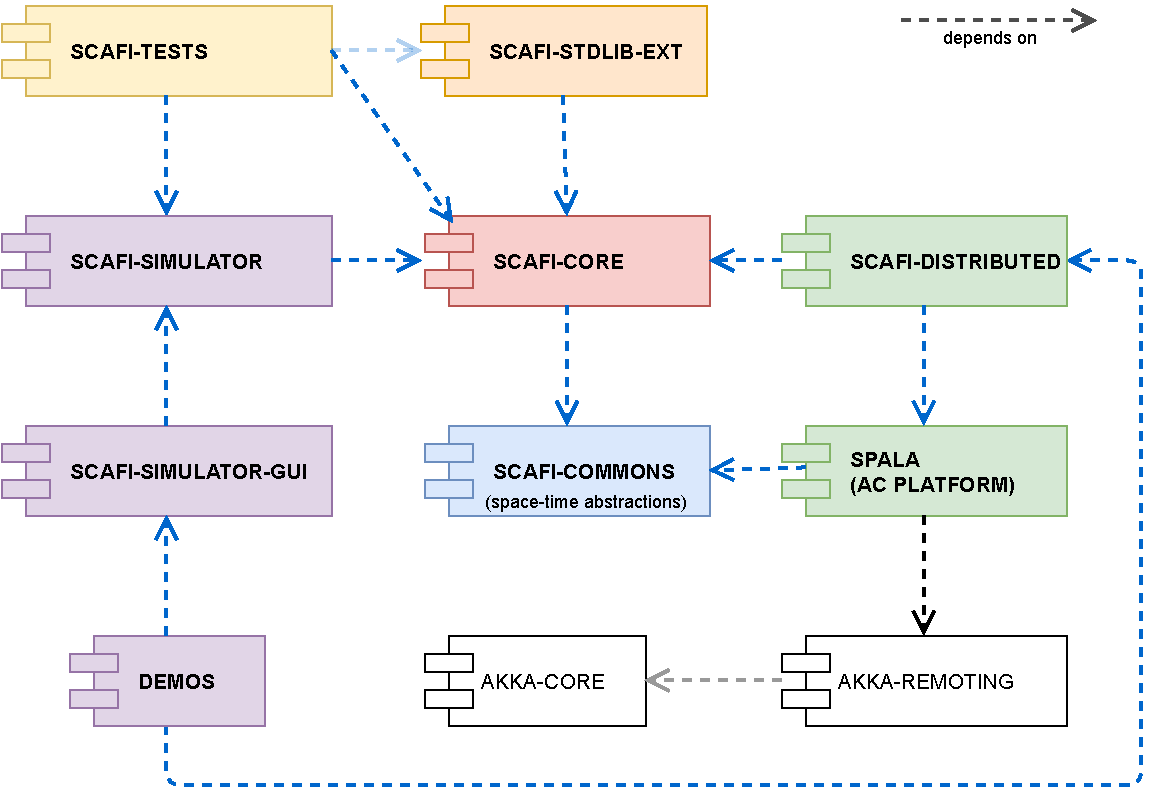
\includegraphics[width=0.8\textwidth]{papers/softwarex2021/imgs/scafi-project-org.pdf}
\caption{High-level architecture of the \scafi{} toolkit.}
\label{fig:scafi-arch}
\end{figure}

\begin{figure}
\centering
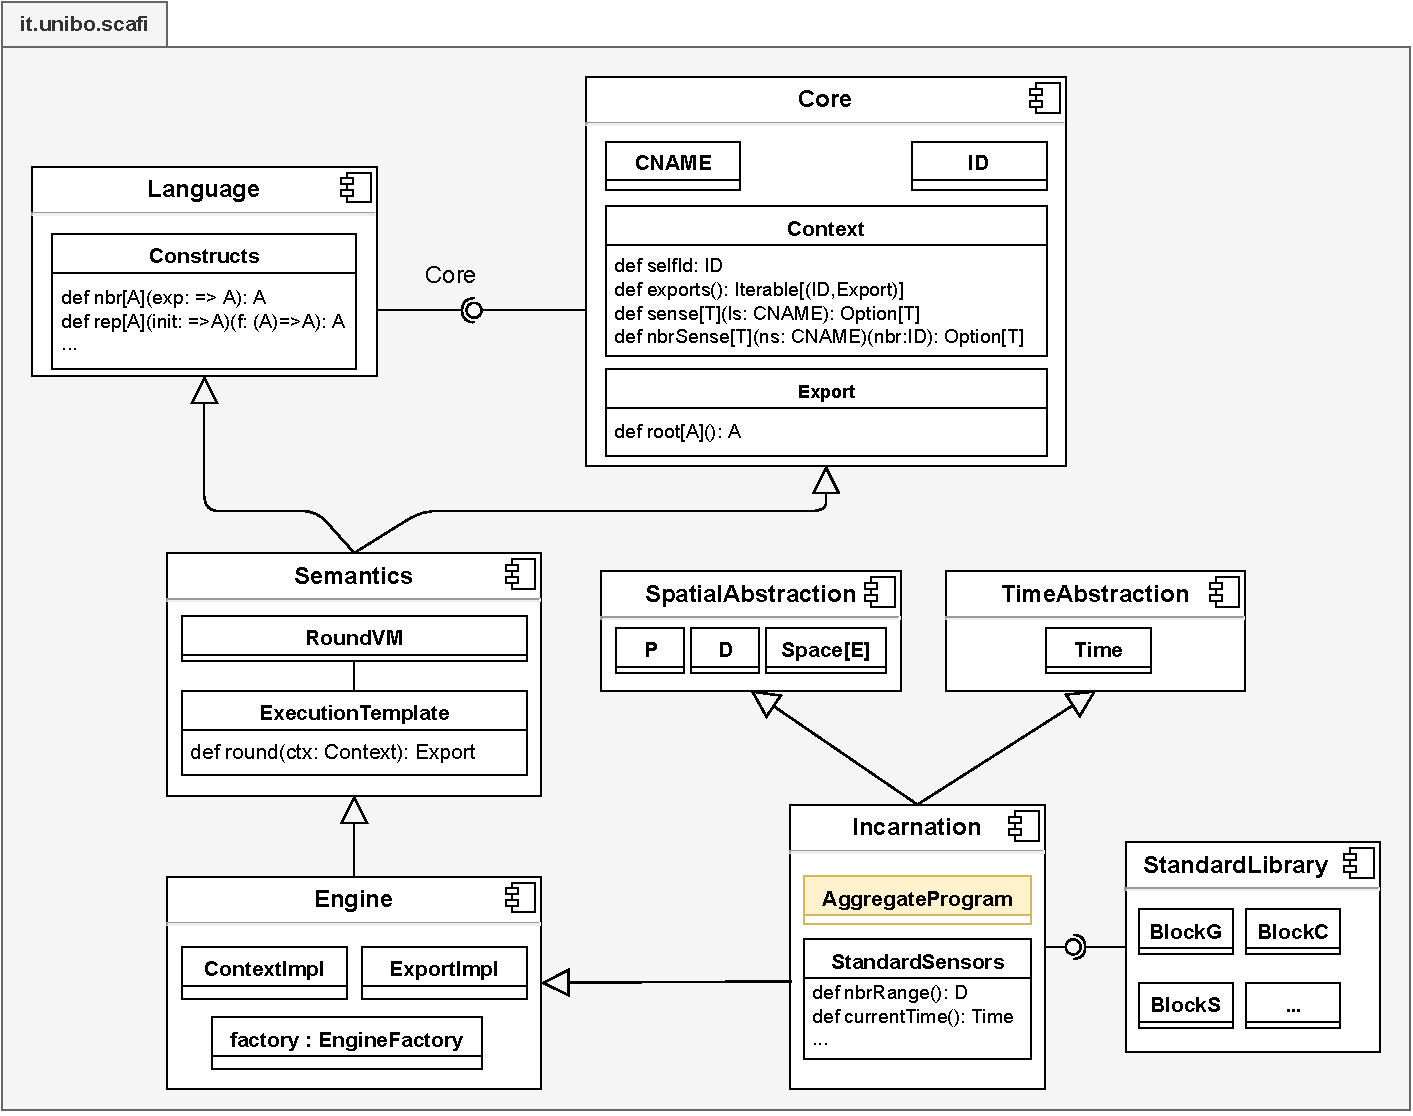
\includegraphics[width=0.8\textwidth]{papers/softwarex2021/imgs/scafi-design.drawio.pdf}
\caption{\revision{Design of the core of \scafi{} (DSL).}}
\label{fig:scafi-design}
\end{figure}

\revision{
\scafi{} leverages the concept of an \emph{incarnation},
 namely a concrete ``family of types''~\cite{DBLP:conf/oopsla/OderskyZ05} 
 that is progressively refined through inheritance, composed, and finally instantiated into an object (cf. the Scala \emph{cake pattern}~\cite{Hunt2013cakepattern,DBLP:conf/oopsla/OderskyZ05})
 which ultimately provides access 
 to a type-coherent set of features.

\Cref{fig:scafi-design} provides an excerpt 
 of the main Scala traits 
 with some types and objects they define.
%
Trait \texttt{Core} provides the abstract fundamental types: \texttt{CNAME} for capability names,
\texttt{ID} for device identifiers,
\texttt{Context} for the input environment of computation rounds,
and \texttt{Export} for the outcomes of computation rounds.
%
Trait \texttt{Language} 
 provides the syntax of the DSL in terms of methods, through interface \texttt{Constructs}.
%
Trait \texttt{Semantics} and \texttt{Engine}
 implement the DSL construct semantics,
 providing a template for \texttt{AggregateProgram} base class defined in the \texttt{Incarnation} trait. 
The incarnation also exposes \texttt{StandardSensors} in terms of, e.g., \texttt{SpatialAbstraction}'s and \texttt{TimeAbstraction}'s types for positions (\texttt{P}), distances (\texttt{P}), and time.
%
The \texttt{StandardLibrary} is provided by leveraging 
 what an incarnation provides,
 providing traits of functionality to be mixed into \texttt{AggregateProgram}s.
}

\paragraph*{Software Functionalities}
\label{}

\subparagraph*{Expressing aggregate programs through a Scala DSL}
\label{sec:express-programs}
%
Module \texttt{scafi-core}
 exposes,
 through incarnations,
 an \texttt{AggregateProgram} trait
  that provides access to 
  aggregate programming constructs---following 
  a variant of the field calculus~\cite{DBLP:journals/tocl/AudritoVDPB19,DBLP:journals/jlap/ViroliBDACP19}
  formalized in~\cite{DBLP:conf/isola/CasadeiVAD20}.
%
This single program defines -- from a global perspective -- 
 the collective adaptive behaviour 
 of an entire %system or 
 ensemble of computational devices.
%
Besides the core constructs,
 this module also provides ``standard library'' traits
 providing access to reusable functions of aggregate functionality.
%
For instance, by mixing trait \texttt{Gradients}
 into an \texttt{AggregateProgram} subclass,
 a developer gets access to \emph{gradient functions}~\revision{\cite{DBLP:conf/sac/BealBVT08,DBLP:journals/tomacs/ViroliABDP18}}, used to 
 continuously compute (over space and time) the self-healing field of minimum distances of each node from a set of source nodes. %---possibly in mobile and faulty environments.
%
Several such traits are available
 to provide other key building blocks
 for self-organising applications~\revision{\cite{DBLP:conf/saso/WolfH07,DBLP:journals/tomacs/ViroliABDP18}} (e.g., \texttt{BlockG} \revision{for gradient-wise information propagation}, \texttt{BlockC} \revision{for gradient-wise information collection}, \texttt{BlockS} \revision{for sparse choice or leader election})
 or experimental language features
 (e.g., the \texttt{spawn} function for concurrent aggregate processes~\revision{\cite{DBLP:journals/eaai/CasadeiVAPD21,testa2022processes}}\revision{, for modelling independent and overlapping aggregate computations}).
%
\subparagraph*{Virtual machine for the local execution of aggregate programs}
%
An \texttt{AggregateProgram} instance 
 is a function
 mapping a \texttt{Context}
 (the set of inputs needed by an individual device
  to properly evaluate the program locally)
 to an \texttt{Export}
 (the tree of values that has to be shared 
  with neighbours to effectively coordinate and promote 
  the emergence of collective behaviours).
%
Using this API,
 a developer can 
 integrate ``aggregate functionality''
 into its system---what remains to be specified are the
 details of the aggregate execution model and the communication among devices,
 that may change in different applications.
%
Devices must continuously run the aggregate program,
but the scheduling of these computation rounds can be tuned
as the application needs~\cite{DBLP:journals/lmcs/PianiniCVMZ21}.
%
\texttt{Export}s must be shared with neighbouring devices to allow them
to properly set up their \texttt{Context}s,
but the network protocol to be used to do so can be selected
independently of the program.
 
\subparagraph*{Simulation support}
%
In order to simulate an ``aggregate system'',
 it is necessary to: 
\begin{enumerate}
  \item define the set of computational devices that make up the aggregate, including their sensors and actuators;
  \item define the aggregate topology, i.e., 
  some application-specific \emph{neighbouring relationship}
  from which the set of \emph{neighbours}
  of each device can be determined;
  \item define the aggregate program to be executed;
  \item define a certain dynamics of the system
  by proper scheduling of computation rounds,
  and the environment
  by proper scheduling of changes in sensor values.
\end{enumerate}

%
Module \texttt{scafi-simulator}
 provides this basic support.
%
It exposes some factory methods
to configure simulations properly
 (e.g., it supports ad-hoc and spatial distance-based connectivity rules)
 and an API to run and interact with simulations.
%
Then, module \texttt{scafi-simulator-gui}
 provides a convenient graphical user interface
 to launch and visually show simulations in execution.
%
We remark that these modules currently support basic simulation scenarios
 and are mainly meant for quick experiments
 or as a starting basis for ad-hoc simulation frameworks.
 
\subparagraph*{Experimental or work-in-progress features: actor-based middleware}
%
Regarding the construction of actual systems, 
 \scafi{}
 provides
 an actor-based implementation
 of the aggregate execution model~\cite{DBLP:series/lncs/CasadeiV18},
 in the \texttt{spala} (\texttt{Spa}tial Sca\texttt{la}) module,
 which is instrumental for integrating aggregate computing
 into existing systems and distributed architectures~\cite{DBLP:series/lncs/CasadeiV18}.
%
Indeed, aggregate computing systems
 can be designed, deployed, and executed 
 according to different
 architectural styles 
 and concrete architectures~\cite{DBLP:journals/fi/CasadeiPPVW20}.
%
So, \scafi{} provides \emph{two} main implementations of the middleware,
 in package \texttt{it.unibo.scafi.distrib.actor},
 for purely peer-to-peer 
 (sub-package \texttt{p2p})
 and server-based designs
 (sub-package \texttt{server}).
%
The main abstraction
 is the \texttt{DeviceActor},
 which exposes a message-based interface
 for controlling and interacting with
 an individual logical node of the aggregate system.
%
Then, an object-oriented façade API is provided to set up a system of middleware-level actors. 

%\subparagraph{Sample code snippets analysis (optional)}
%\label{}

%\subparagraph{Illustrative Examples}
\paragraph*{Features}
\label{s:impact}
\scafi{}
 has been used 
 in aggregate computing-related research~\cite{DBLP:journals/eaai/CasadeiVAPD21,audrito2022ecoop-xc,DBLP:conf/coordination/AguzziCV22,
 DBLP:conf/fmec/CasadeiV19,DBLP:conf/IEEEscc/CasadeiTVD19,DBLP:journals/scp/CasadeiAV18,DBLP:journals/jsan/CasadeiAV21,DBLP:conf/coordination/CasadeiVRA21,casadei2022applsci,arxiv2020scafi-nc},
  touching themes such as 
  software engineering, 
  computational models, and
  distributed systems/algorithms.
%
The impact of \scafi{}
 can be understood in terms of 
 existing and prospective contributions, 
 discussed in the following.

\subparagraph*{Interplay between programming language design and foundational research} 
%
The implementation of the \scafi{} DSL
 has inspired a variant of the field calculus
 which arguably supports easier embeddability
 into mainstream programming languages~\cite{DBLP:conf/isola/CasadeiVAD20,arxiv2020scafi-nc}.

\subparagraph*{High-level programming models}
%
The previous discussion  
 makes the case for ``DSL stacking''~\cite{DBLP:conf/icsoft/HummE10}.
%
Indeed, by leveraging the aforementioned aggregate process extension, 
 it is possible to reduce the abstraction gap
 needed to implement \emph{situated tuples}~\cite{DBLP:conf/coordination/CasadeiVRA21}\revision{,
 which is a Linda-like model~\cite{DBLP:journals/toplas/Gelernter85} for coordinating processes where tuples and tuple operations are situated in space}.
%
By mapping high-level specifications into aggregate programs, it is sometimes straightforward to develop resilient distributed implementations---as in~\cite{DBLP:journals/jss/AudritoCDSV21},
 where translation rules from 
 spatial logic formulas
 to field calculus expressions
 enable seamless construction of decentralized monitors for such formulas.

\subparagraph*{Web-friendliness}
%
By leveraging Scala.js~\cite{DBLP:conf/scala/Doeraene18}, \scafi{} can be easily 
 accessed through JavaScript,
 which promotes cross-platform language design 
 and reuse of functionality in the browser
 (to support web applications without the need of server-side components).
%
This paved the path 
 to \scafiweb{}~\cite{DBLP:conf/coordination/AguzziCMPV21},
 a web playground for aggregate programming.
%
\section{Software Description}\label{coordination2023:contribution}
\scarlib{} \footnote{Tool available on GitHub at \url{https://github.com/ScaRLib-group/ScaRLib}}~\footnote{demo video at: \url{https://github.com/ScaRLib-group/ScaRLib-demo-video}} is a research Scala framework designed to support
the development of \ac{MAARL} systems by JVM-based high-level specification, and with learning performed under the hood by PyTorch\footnote{\url{https://pytorch.org/}}.
%
This project aims to provide a tool that allows easy and powerful system specification.
%
To meet this purpose we have designed many abstractions, that model high-level aspects of the \ac{MAARL} domain, 
 without caring about low-level implementation details.
Basically, \scarlib{} is composed of three main modules (\Cref{coordination2023:fig:modules}), namely: 
\begin{itemize}
    \item \texttt{scarlib-core} that implements the main abstractions over the \ac{MAARL} domain,
    \item \texttt{dsl-core} that provides a high-level language to specify the system, and
    \item \texttt{alchemist-scafi} that provides bindings between \scarlib{} and the two tools Alchemist and \scafi{}.
    It is important to note that \scarlib{} is not limited to the Alchemist-\scafi{} combination, that module is 
    already implemented due to the actual need, however, it is possible to implement other bindings to other tools
    (e.g., by replacing Alchemist with some other simulator, for example, FLAME GPU~\cite{flame}).
\end{itemize}
\begin{figure}[t]
    \centering
    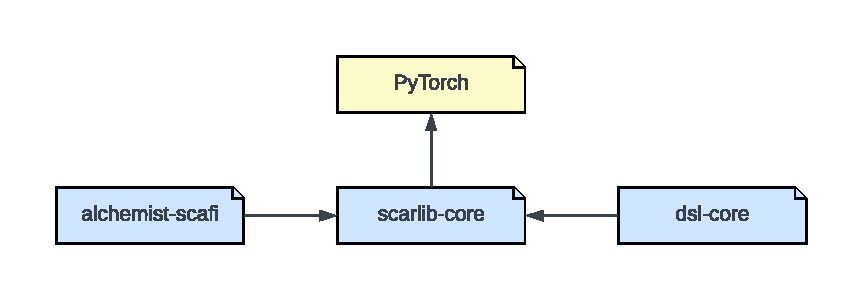
\includegraphics[width=0.7\textwidth]{papers/coordination2023/imgs/scarlib-modules.pdf}
    \caption{\scarlib{} main modules}
    \label{coordination2023:fig:modules}
\end{figure}

\subsection{Core abstraction} The module \texttt{scarlib-core} implements the core functionalities and abstractions of the framework, 
such as the definition of the main data structures and the implementation of the main algorithms. 
%
All the abstractions (\Cref{coordination2023:fig:arc}) are built around a bunch of concepts. 
 The key element is the \texttt{System}, 
 which is a collection of agents that interact within a shared environment and that are trained to optimize a global or local reward signal
expressed by a reward function. 
%
The tool comes with two types of systems already implemented that are very common in literature~\cite{Du2020},
i.e., centralized training and decentralized execution (\texttt{CTDESystem}) and decentralized training and execution (\texttt{DTDESystem}).
Furthermore, an implementation of the DQN algorithm \cite{Mnih2015} is provided and used to train agents. 
The end-user who wants to run a learning process only has to implement four elements
in order to define his own system with the desired \emph{collective} goal, which are:
\begin{enumerate}
    \item the \emph{environment}: that is the place where the agents live, 
    \item the \emph{agent state space}: namely the information that the agent can perceive from the environment, 
    \item the \emph{action space}: namely the actions that the agent can perform in that environment, and
    \item the \emph{reward function}: that is the function that the agent has to maximize.
\end{enumerate} 
Only by using this module, 
 it is possible to run a simple learning process in a simulated environment based on our platform.

\begin{figure}[t]
    \centering
    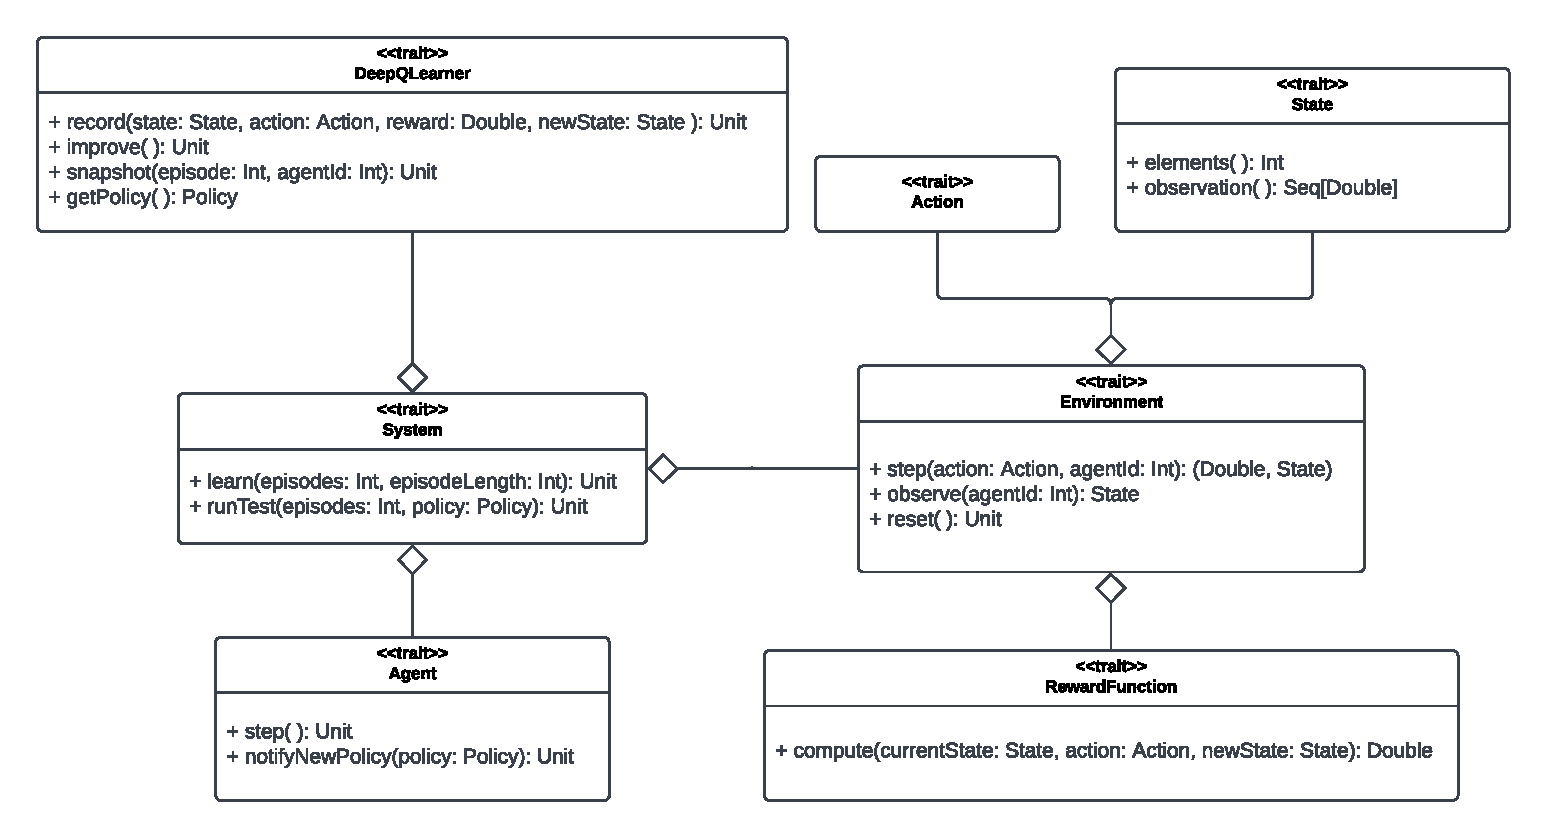
\includegraphics[width=\textwidth]{papers/coordination2023/imgs/core-architecture.pdf}
    \caption{\scarlib{} core architecture}
    \label{coordination2023:fig:arc}
\end{figure} 
To gain a deeper comprehension of the system dynamics, 
 a discussion of the underlying mechanisms is warranted.
%
Both systems employ a training algorithm characterized by a sequence of \emph{epochs}, 
 each encompassing a collection of \emph{episodes}.
Within each episode, 
 agents are presented with the current state, which serves as an input for action selection.
%
The collective action executed by the agents prompts a state transition in the environment, 
 thereby facilitating the progression to the subsequent episode.
Upon completion of an epoch, the environment is reinitialized, 
 and the agents undergo training based on the aggregated experience.

Most specifically,
 if the chosen system is a \texttt{CTDESystem} (\Cref{coordination2023:fig:ctde}) the agents are trained in a centralized way, 
 for that reason, there is  a single central dataset, 
 where the global experience of all the agents is stored, 
 and a single central learner that is responsible for the training process 
 and for the improvement of the policy neural network.
% 
The system is also responsible 
 for the execution of all the agents and the notification of the updated policy.
% 
In this way, it is possible to easily extend the system in order to modify the execution flow, e.g., 
 if a concurrent and distributed execution is needed. 
%
The \texttt{DTDESystem} (\Cref{coordination2023:fig:dtde}) works similarly, 
 the only difference is that every agent has its own dataset and learner.

%In order to provide an efficient learning process we have bindings with a state-of-the-art 
% deep learning library, namely: PyTorch \footnote{\url{https://pytorch.org/}}.
% Those bindings are provided by another library called ScalaPy \footnote{\url{https://scalapy.dev/}} 
% and allows the end-user to train the models both on CPUs and GPUs.

Regarding the training process,
 since the tool aims to support neural-network-based RL algorithms (like DQN),
 we chose to use the current de facto standard framework 
 for building neural networks, which is PyTorch---alternatives include DL4J~\footnote{\url{https://deeplearning4j.konduit.ai/}}, which could be subject of future investigation.
 
%
One way to integrate this library into a JVM environment could be 
 to rely on its native core (LibTorch) using Java Native Interface (JNI) -- 
 as was done in \texttt{scala\_torch}~\footnote{\url{https://github.com/microsoft/scala_torch}} project. 
 In \scarlib{}, we chose a convenient approach 
 that allowed us not only to access PyTorch 
 but also all the libraries connected to it 
 (e.g., torch geometric, etc.), 
 which is to use ScalaPy~\cite{Laddad2020}  to interact directly with the Python API 
 of these libraries.
%
This integration generally involves:
\begin{enumerate}
    \item setting up a Python environment in which the libraries of interest are instantiated;
    \item creating a Scala API that isolates what is necessary to access the Python ecosystem.
\end{enumerate}
In this case, we have isolated everything in DQN, 
 which is therefore the entry point for accessing PyTorch.
\begin{figure*}[t]
    \centering
    \begin{subfigure}[b]{0.49\textwidth}
        \centering
        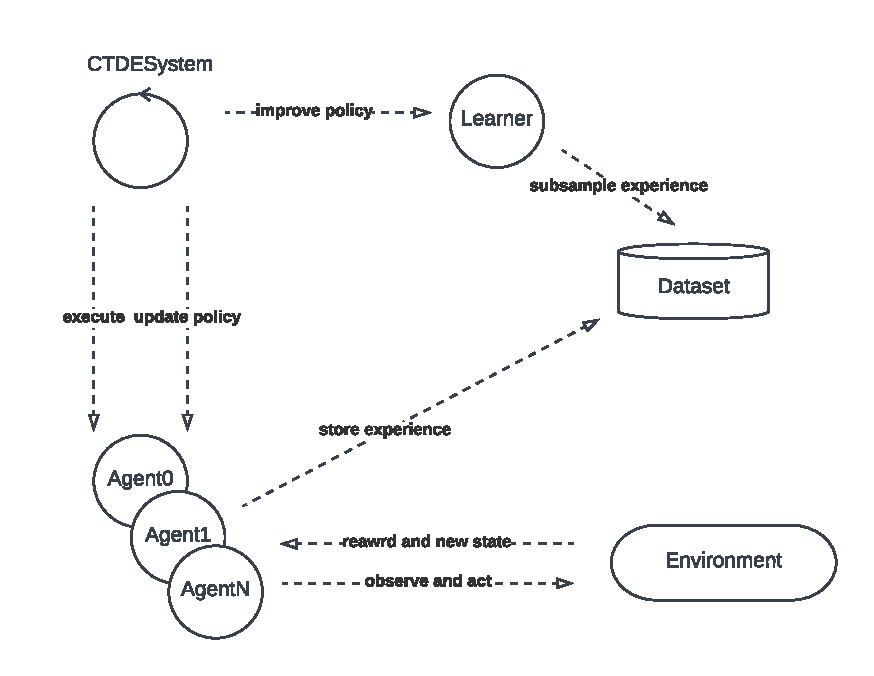
\includegraphics[width=\textwidth]{papers/coordination2023/imgs/ctdesystem.pdf}
        \caption{CTDE System}
        \label{coordination2023:fig:ctde}
    \end{subfigure}
    \begin{subfigure}[b]{0.49\textwidth}
        \centering
        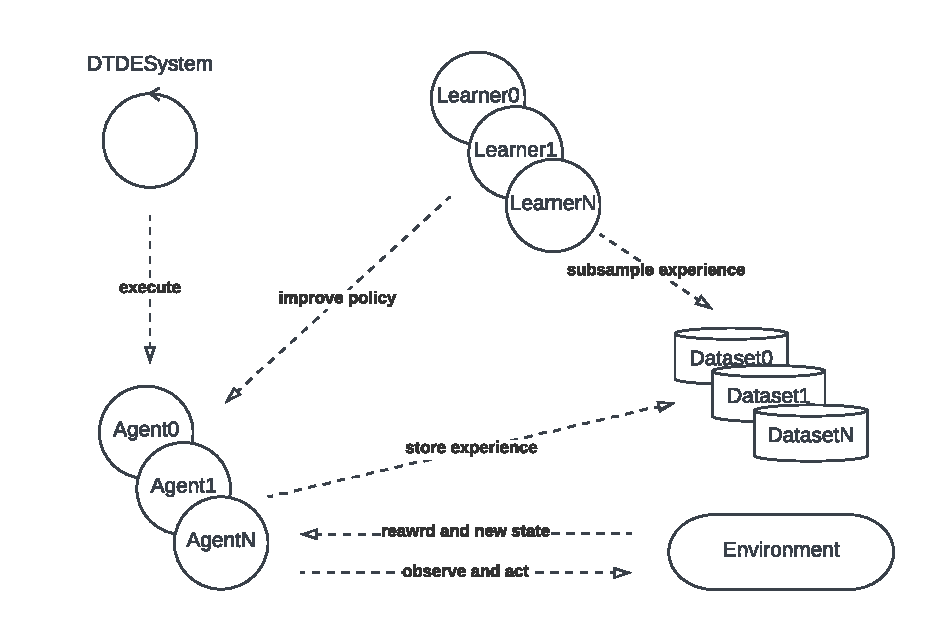
\includegraphics[width=\textwidth]{papers/coordination2023/imgs/DTDE.pdf}
        \caption{DTDE System}
        \label{coordination2023:fig:dtde}
    \end{subfigure}
\caption[Examples of developed System dynamics in \scarlib{}]{Examples of developed system dynamics. 
On the left, there is the centralized system, 
where a learner with a global view of the system 
updates the policy shared with all agents. 
%
On the right, there is a decentralized system, 
where each agent has a local policy and a local policy.}
\end{figure*}

\subsection{\scafi{}-Alchemist integration} In addition to the core, 
 we have implemented another module called \texttt{alchemist-scafi} (\Cref{coordination2023:fig:alchemist-arc}) 
 in which there is the integration with the two tools: 
 Alchemist and \scafi{}.
%
Such integration enables the possibility to run the learning process 
 in an aggregate computing context.
This is a key part of this contribution. 
 In fact, although Alchemist has been used for cooperative many-agent reinforcement learning with \scafi{} as shown in previous chapters, 
 ad-hoc solutions were always created that were difficult to \emph{reuse}, 
 \emph{rigid}, \emph{untested}, and had \emph{interoperability issues} between Alchemist 
 and the chosen native libraries.
With this integration, 
 we aim to deliver a robust and user-friendly system that will serve as a long-term solution, 
 fostering greater engagement within the multi-agent reinforcement learning community. 
 This simulator and paradigm have already demonstrated their versatility in representing a wide range of environments, as discussed in \Cref{part:background}.

The specification of a learning system does not change, only two new elements are added: 
 the specification of the Alchemist simulation and the implementation of the \scafi{}-based logic.
%
Specifically, 
 the Alchemist simulation is configured as depicted in \Cref{coordination2023:fig:alchemist}, 
 where a \scafi{} class, encapsulating the aggregate programming code, is passed as a program. 
 To facilitate the training progression, a molecule containing the current action--a subclass of the \texttt{Action} class--is integrated within the \scafi{} program. 
 This molecule is injected by a learner governing the \ac{rl} policy. Additionally, the aggregate program evaluates the environment state, which is required to be a subtype of the \texttt{State} class, 
 via the \texttt{computeState} method. 
 This computed state is subsequently encapsulated in the \texttt{state} molecule, serving as input for the learner to refine the policy.
\begin{figure}[t]
    \centering
    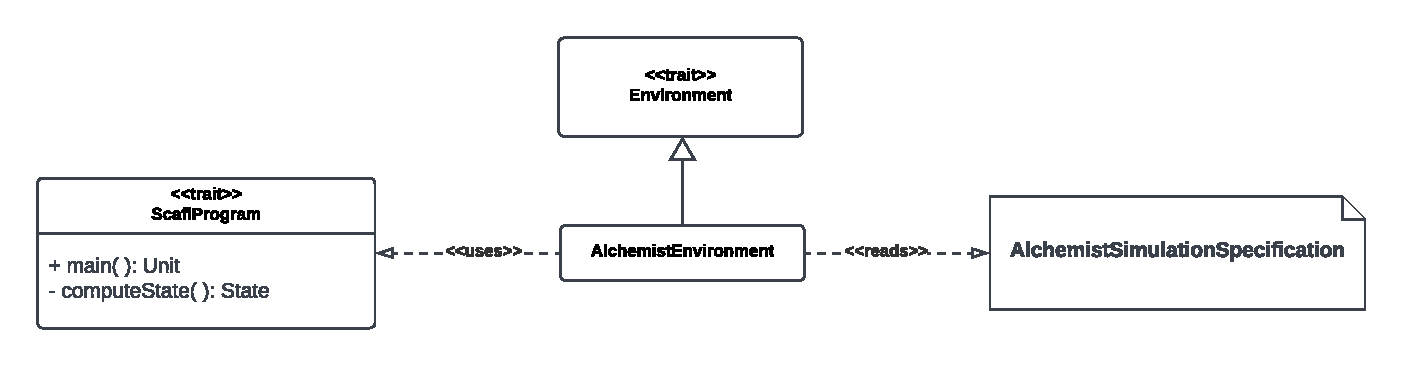
\includegraphics[width=\textwidth]{papers/coordination2023/imgs/alchemist-scafi-arc.pdf}
    \caption[\scarlib{} \texttt{alchemist-scafi} architecture]{\scarlib{} \texttt{alchemist-scafi} architecture. 
    A \texttt{ScafiProgram} should be passed to the \texttt{AlchemistEnvironment}
    in order to start the learning process. 
    }
    \label{coordination2023:fig:alchemist-arc}
\end{figure}

\subsection{DSL for learning configurations} 
Finally, we developed an internal \ac{dsl} designed to streamline the development of \ac{MAARL} training systems. 
 This approach aims to seamlessly translate the concepts envisioned by a \ac{MAARL} system designer into a functional training system. 
 Utilizing a strongly-typed language like Scala for our DSL enables error detection at compile-time, 
 thereby preempting simple configuration errors that might otherwise only be caught during runtime.

The public-facing DSL serves as a simplified interface to the underlying abstractions encapsulated in the \texttt{scarlib-core} module. 
 Consequently, when a developer wishes to initiate a simulation 
 (for example, in Alchemist), 
 they must first specify a reward function. 
 This function serves as a metric for evaluating the performance of a particular agent in relation to the current state of the environment.

\begin{lstlisting}
class MyRewardFunction extends CollectiveRewardFunction:
    override def computeReward(
        state: State, 
        action: Action, 
        nextState: State
    ): Double = ...
\end{lstlisting}
Consequently, they must decide which actions are supported 
 by the agents living in the chosen system. 
%
Since we are talking about \ac{MAARL} systems, 
 we suppose that each agent has the same action space. 
 Thus, it is possible to define a set of actions as a product type:
\begin{lstlisting}
sealed trait MyAction extends Action
object MyAction:
    case object A extends MyAction
    case object B extends MyAction
    case object C extends MyAction
    def all: Seq[MyAction] = Seq(A, B, C)
\end{lstlisting}
Final refinements required include: 
\begin{itemize}
    \item choosing the class of the Alchemist environment to instantiate, 
    \item defining the number of agents living in the chosen environment, and 
    \item defining the size of the buffer in which the memory will be stored.
\end{itemize}
This can be expressed as follows:
\begin{lstlisting}
val system = learningSystem {
    rewardFunction { new MyRewardFunction() }
    actions { MyAction.all}
    dataset { ReplayBuffer[State, Action](10000) }
    agents { 50 } // select the number of agent
    environment {
        // select a specific environment
        "it.unibo.scarlib.experiments.myEnvironment"
    }
}
\end{lstlisting}

\subsection{Tool usage}
The tool is published on Maven Central 
 and it is possible to include it in your project, 
 for example, through a build system. 
 In the case of Gradle, for instance, 
 you will need to add the following instructions:
\begin{lstlisting}
implementation("io.github.davidedomini:scarlib-core:1.5.0")
implementation("io.github.davidedomini:dsl-core:1.5.0")
\end{lstlisting}
%
At this point, it will be possible to create 
 your own training system as shown in the DSL section. 
 To start the training, you will then need to write:
\begin{lstlisting}
learningSystem.train(episodes = 1000, episodeLength = 100)
\end{lstlisting}
%
Of course, 
 the system can also be used to verify a certain 
 policy that has been learned during a training process. 
% 
To do this, first, 
 you will need to load the neural network extracted during training:
\begin{lstlisting}
val network = PolicyNN(path, inputSize = ..., hiddenSize = ...)
\end{lstlisting}
Then you can execute the test in the following way:
\begin{lstlisting}
system.runTest(episodeLength = 100, network)
\end{lstlisting}
For further details on how to specify simulations and environments, 
 please refer to the repository README, 
 the presentation video and 
 the developed simulation (following section).
\section{Experiments}\label{coordination2023:experiments}
% \meta{This section should provide a description of the experiments, including the results and the discussion.}
% \meta{For each experiment, we can have the following structure:
% \paragraph{Description}
% Here you should describe the experiment, including the environment, the agents, the algorithm, etc.
% \paragraph{Results}
% Here you should show the result of the experiment, including the plots and the discussion.
% }

%\subsection*{Cohesion and Collision}
\subsection{Description}
%This environment consists of a group of agents (in our experiment fifty) that interact in a 2D world 
% to learn how to stay close with each other without colliding. 
%Each agent has a fixed neighborhood (the three closest, that is an hyper-parameter) 
% and can perform eight actions, namely: north, south, east, 
% west, north-east, north-west, south-east and south-west. 
% The state of each agent consist of the relative distance to the neighborhood 
%  and of his own position.
%The reward function (\Cref{coordination2023:fig:cc-rf}) is parametrized by a target distance $d$, in the graph the target
% distance is represented by the red vertical line.
% The portion of the graph to the right of the red line represents the influence of the cohesion term:
% the more the agents are far from each other, the more the reward linearly decrease.
% Instead, the portion of the graph to the left of the red line represents the influence of the 
% collision term: if the agents are too close to each other, the reward function 
% has an exponential decreasing trend. 
To test ScarLib's functionality, 
 we develop an experiment~\footnote{repository available at \url{https://github.com/ScaRLib-group/ScaRLib-flock-demo}}
 involving a relatively large number of agents 
 and non-trivial coordination tasks. 
% 
We aim to create a flock of drones 
 that moves to avoid collisions with each others, by learning a policy by which each 
 agents decide how to move based on neighbours relative position.
% 
This is a well-known problem, and various models and algorithms exist which we draw upon \cite{DBLP:conf/siggraph/Reynolds87,inverserl}. %% todo add citations
% and learning processes exist. % I'd try not to say this... or just discuss it in related works
%
In this case, %%
 we assumed that agents position themselves in an unlimited 2D environment 
 with a fixed neighbourhood (the closest five, in our experiments, though this is a simulation parameter)
 and have the ability to perform movement steps in the 8 directions of a square grid (horizontally, vertically, or diagonally).
%
The environment state, as perceived by the single agent, is the relative distance to the closest neighbours.
%
Particularly, it was expressed through \scafi{} as:
\begin{lstlisting}
val state = foldhoodPlus(Seq.empty)(_ ++ _)(Set(nbrVector))
\end{lstlisting}
where \texttt{nbrVector} is the vector representing the relative position of the neighbour.
\lstinline|foldhoodPlus| is a \scafi{} function that allows to fold over the neighbourhood 
 and \lstinline|++| is the concatenation operator for sequences.

The crucial point for this task is
 the definition of the reward function. 
 In this simulation, we based it on \emph{collision} and \emph{cohesion} factors. 
%
We aim to learn a policy by which agents, initially spread in a very sparse way in the environment, move toward each other until reaching approximate $\delta$  distance without colliding, ultimately forming one or many close groups.
%
%Most specifically, the action taken by an agent is expressed as a movement towards the (closest) neighbour with maximum distance: what we want to learn is the distance to be travelled.

The collision factor comes into play when the distance is less than $\delta$, 
 and exponentially weighs the distance $d$ relative to its closest neighbour:
\begin{equation}
    \label{coordination2023:eq:collision-factor}
    \begin{split}
        \text{collision} = \begin{cases}
            0 & \text{if } d > \delta \\
            \exp\left(-\frac{d}{\delta}\right) & \text{otherwise}
        \end{cases}
    \end{split}
\end{equation}
In this way, when the negative factor is taken into account: 
 the system will tend to move nodes away from each other.

However, if only this factor were used, 
 the system would be disorganized. 
 This is where the cohesion factor comes in. 
 Given the neighbour with the maximum distance $D$, 
 it linearly adjusts the distance relative to the node being evaluated by function:
\begin{equation}
    \text{cohesion} = \begin{cases}
        0 & \text{if } d < \delta \\
        -(D - \delta) & \text{otherwise}
    \end{cases}
\end{equation}
%
The overall reward function is defined as the sum of these two factors ($cohesion + collision$)
 as shown in \Cref{coordination2023:fig:cc-rf}.
 \begin{figure}[t]
    \centering
    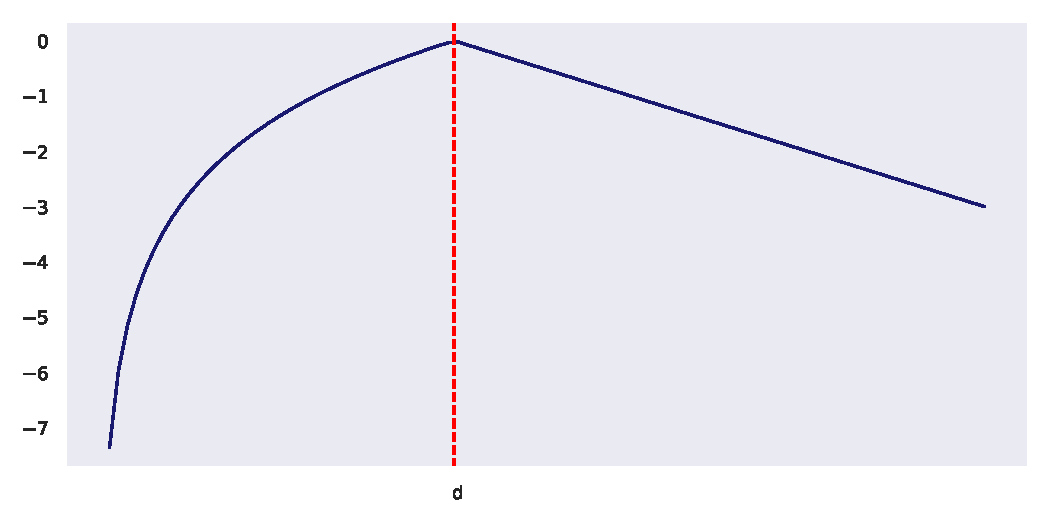
\includegraphics[width=0.6\textwidth]{papers/coordination2023/imgs/ccreward.pdf}
    \caption[cohesion collision reward function]{Cohesion-Collision reward function: the red vertical line represents the target distance $d$.
        The portion of the graph to the right of the red line represents the influence of the cohesion term,
        while the left one represents the influence of the collision term.
    }
    \label{coordination2023:fig:cc-rf}
\end{figure}


\subsection{Results}
%\Cref{coordination2023:fig:cc-results} shows the results of the two experiments, the first one ran with 25 agents (purple lines)
%    and the second one with 50 agents (cyan lines) using a hundred and fifty episodes each of two hundred steps.
% The first graph (\Cref{coordination2023:fig:loss-cc}) shows a comparison of the loss functions,
%  while the second one of the reward functions. 
%  In both learning processes, 
%  when the loss function increases, 
%  the reward function decreases, 
%  which is to be expected as they are inversely proportional. Additionally, both cases exhibit similar 
%  inflexion points despite differences in the agents used, and convergence is achieved in both cases after around 
%  75 episodes.
%  The results are consistent with the predictions and the outcome 
%  does not vary significantly with a different number of agents.
To verify the functionality of the described simulation, 
 we divided the evaluation into two parts. 
%
In the first part, 
 we trained the system for a total of 1000 epochs, 
 each consisting of 100 episodes (or steps). 
%
For each epoch,
 we randomly place 50 agents in a grid large 50x50 meters.
 We set the target distance $\delta$ at 2 meters.

Given the flexibility of \scarlib{}, 
 we tested the training with both CDTE and DTDE processes 
 to ensure that the system could produce policies 
 capable of solving the described task in both cases. 
% 
With the homogeneous policies found (i.e., the one extracted from the CTDE process), 
 we verified that the system's behaviour 
 was consistent with what was learned by varying the initial seed 
 in 16 simulations.
%
With the CDTE policy, 
 since we considered the system homogeneous, 
 we also verified the behaviour as the number of nodes varied,
 expecting similar performance as the nodes increased.

The graphs shown in \Cref{coordination2023:fig:cc-results} 
 demonstrate the \emph{multi-objective} nature of the problem. 
In fact, cohesion and collision are two contrasting signals, 
 and the system had to find a balance between these two values. 
 The graphs show that DQN can generally optimize one signal at a time, 
 with cohesion tending towards zero and collision increasing. 
% 
Nonetheless, after 500 epochs in CTDE simulation,  
 we see that the system had already found a balance between these two factors.
%
In the case of DTDE learning, 
 we observe that convergence is achieved in fewer steps (\~ 50). 
 This is because there is a greater number of policies and 
 therefore greater overall complexity compared to a single homogeneous policy.

During the testing phase 
 (\Cref{coordination2023:fig:simulation-snapshots} shows a series of snapshots of the learned policy), 
 we observed that the system is capable of maintaining a distance of approximately $\delta$, 
 both in the CDTE and DTDE cases. 
 Most specifically, 
 we note that the homogeneous policy is generally 
 a winning choice for homogeneous \ac{MAARL} tasks. 
%
Increasing the number of agents (from 50 to 200), 
 we can observe that collective performances are similar to those with few agents (\Cref{coordination2023:fig:test}).
\begin{figure*}[t]
    \centering
    \begin{subfigure}[b]{0.32\textwidth}
        \centering
        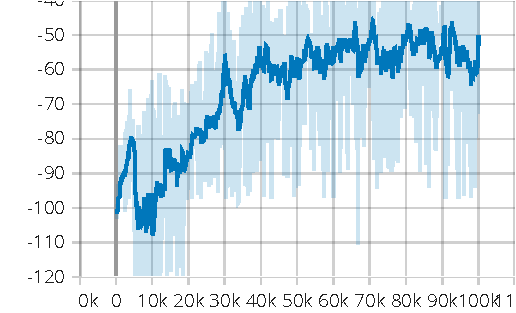
\includegraphics[width=\textwidth]{papers/coordination2023/imgs/reward-ctde.pdf}
        %\caption{Total average reward}
        %\label{coordination2023:fig:reward-cc}
    \end{subfigure}
    \hfill
    \begin{subfigure}[b]{0.32\textwidth}
        \centering
        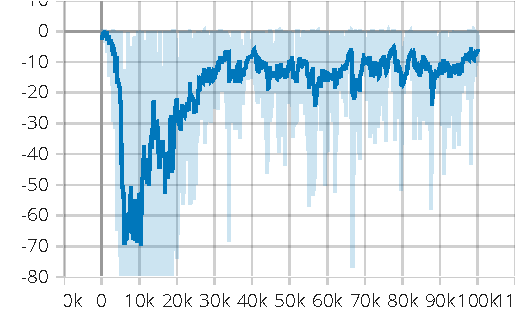
\includegraphics[width=\textwidth]{papers/coordination2023/imgs/collision-ctde.pdf}
        %\caption{Average collision factor}
        %\label{coordination2023:fig:collision-cc}
    \end{subfigure}
    \hfill
    \begin{subfigure}[b]{0.32\textwidth}
        \centering
        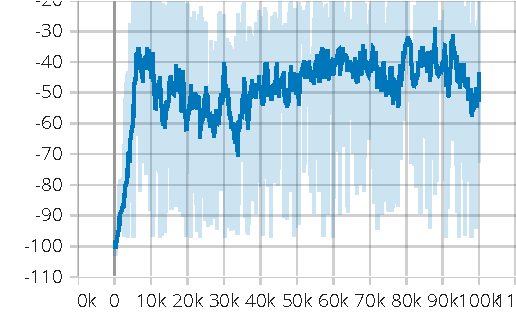
\includegraphics[width=\textwidth]{papers/coordination2023/imgs/cohesion-ctde.pdf}
        %\caption{Average cohesion factor}
        %\label{coordination2023:fig:cohesion-cc}
    \end{subfigure}
    \par\bigskip
    \begin{subfigure}[b]{0.32\textwidth}
        \centering
        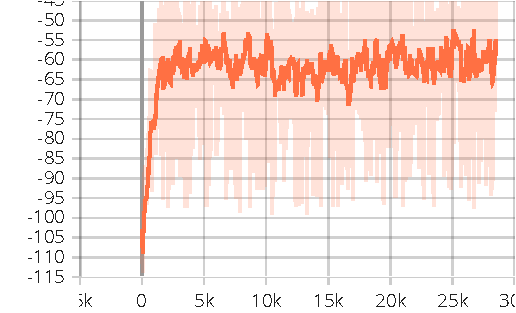
\includegraphics[width=\textwidth]{papers/coordination2023/imgs/reward-dtde.pdf}
        \caption{Total average reward}
        \label{coordination2023:fig:reward-dcc}
    \end{subfigure}
    \hfill
    \begin{subfigure}[b]{0.32\textwidth}
        \centering
        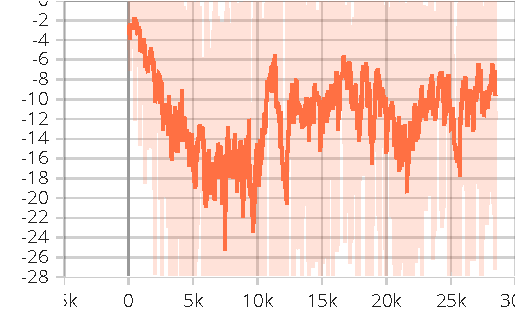
\includegraphics[width=\textwidth]{papers/coordination2023/imgs/collision-dtde.pdf}
        \caption{Average collision factor}
        \label{coordination2023:fig:collision-dcc}
    \end{subfigure}
    \hfill
    \begin{subfigure}[b]{0.32\textwidth}
        \centering
        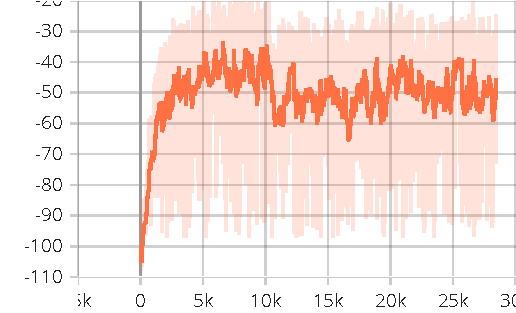
\includegraphics[width=\textwidth]{papers/coordination2023/imgs/cohesion-dtde.pdf}
        \caption{Average cohesion factor}
        \label{coordination2023:fig:cohesion-dcc}
    \end{subfigure}
\caption[Cohesion and collision experiment results]{Cohesion and collision experiment results. The y-axis represents the reward value.
The x-axis represents the total number of episodes.
The first three graphs show the results of the CDTE learning process, while the last three show the results of the DTDE learning process.}
\label{coordination2023:fig:cc-results}
\end{figure*}

\begin{figure*}[t]
    \centering
    \begin{subfigure}[b]{0.25\textwidth}
        \centering
        \fbox{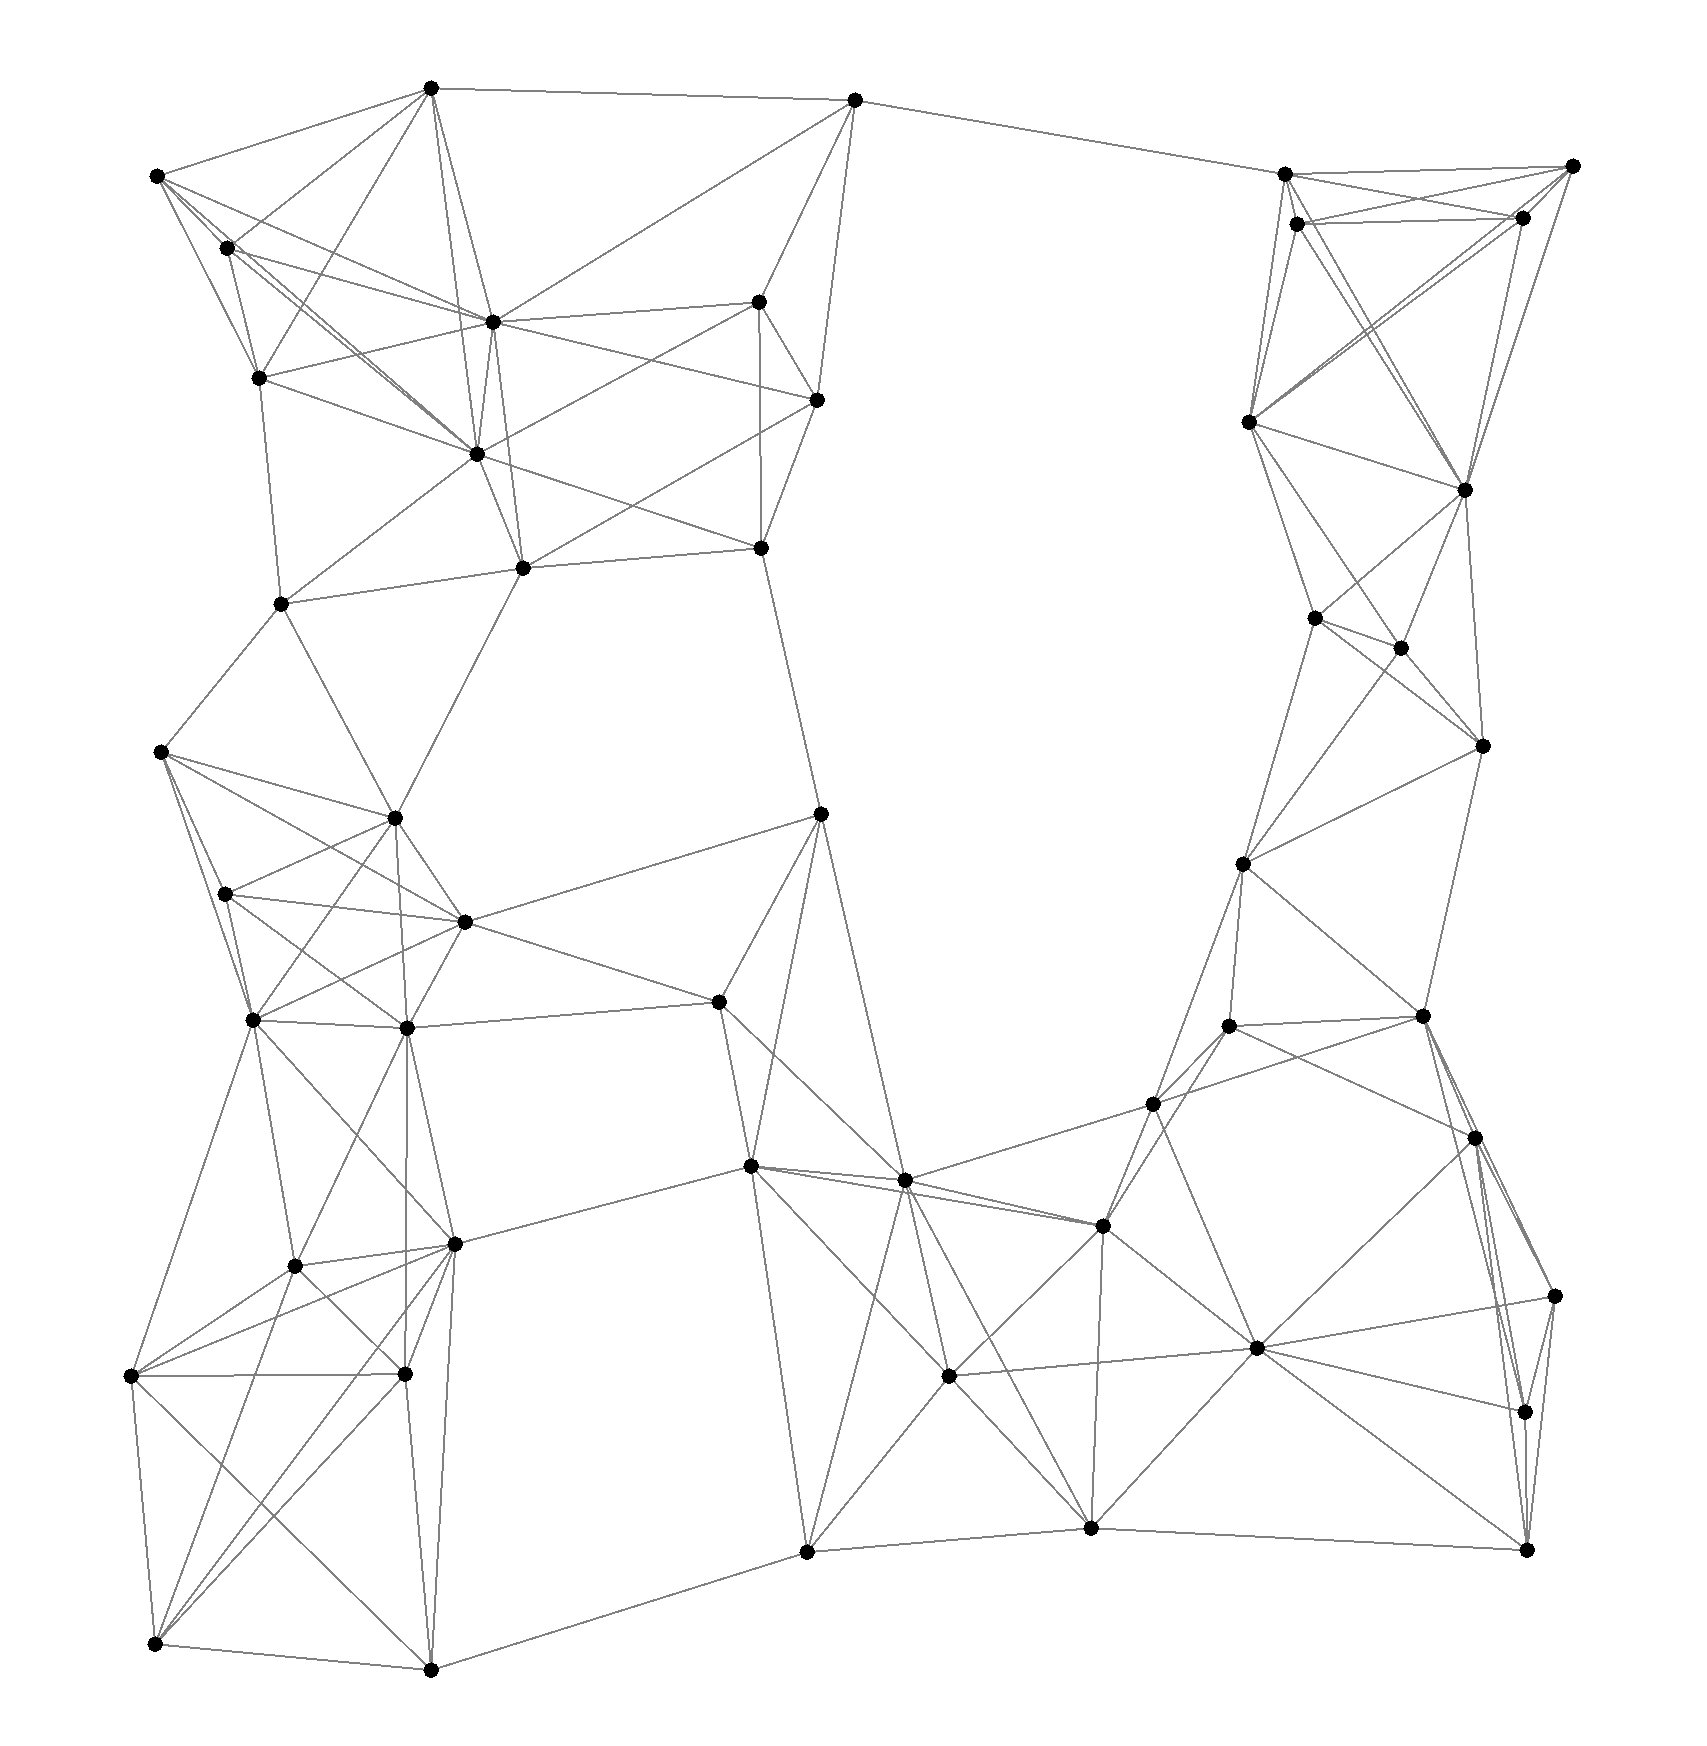
\includegraphics[width=\textwidth]{papers/coordination2023/imgs/1.png}}
        \caption{}
    \end{subfigure}
    \hfill
    \begin{subfigure}[b]{0.25\textwidth}
        \centering
        \fbox{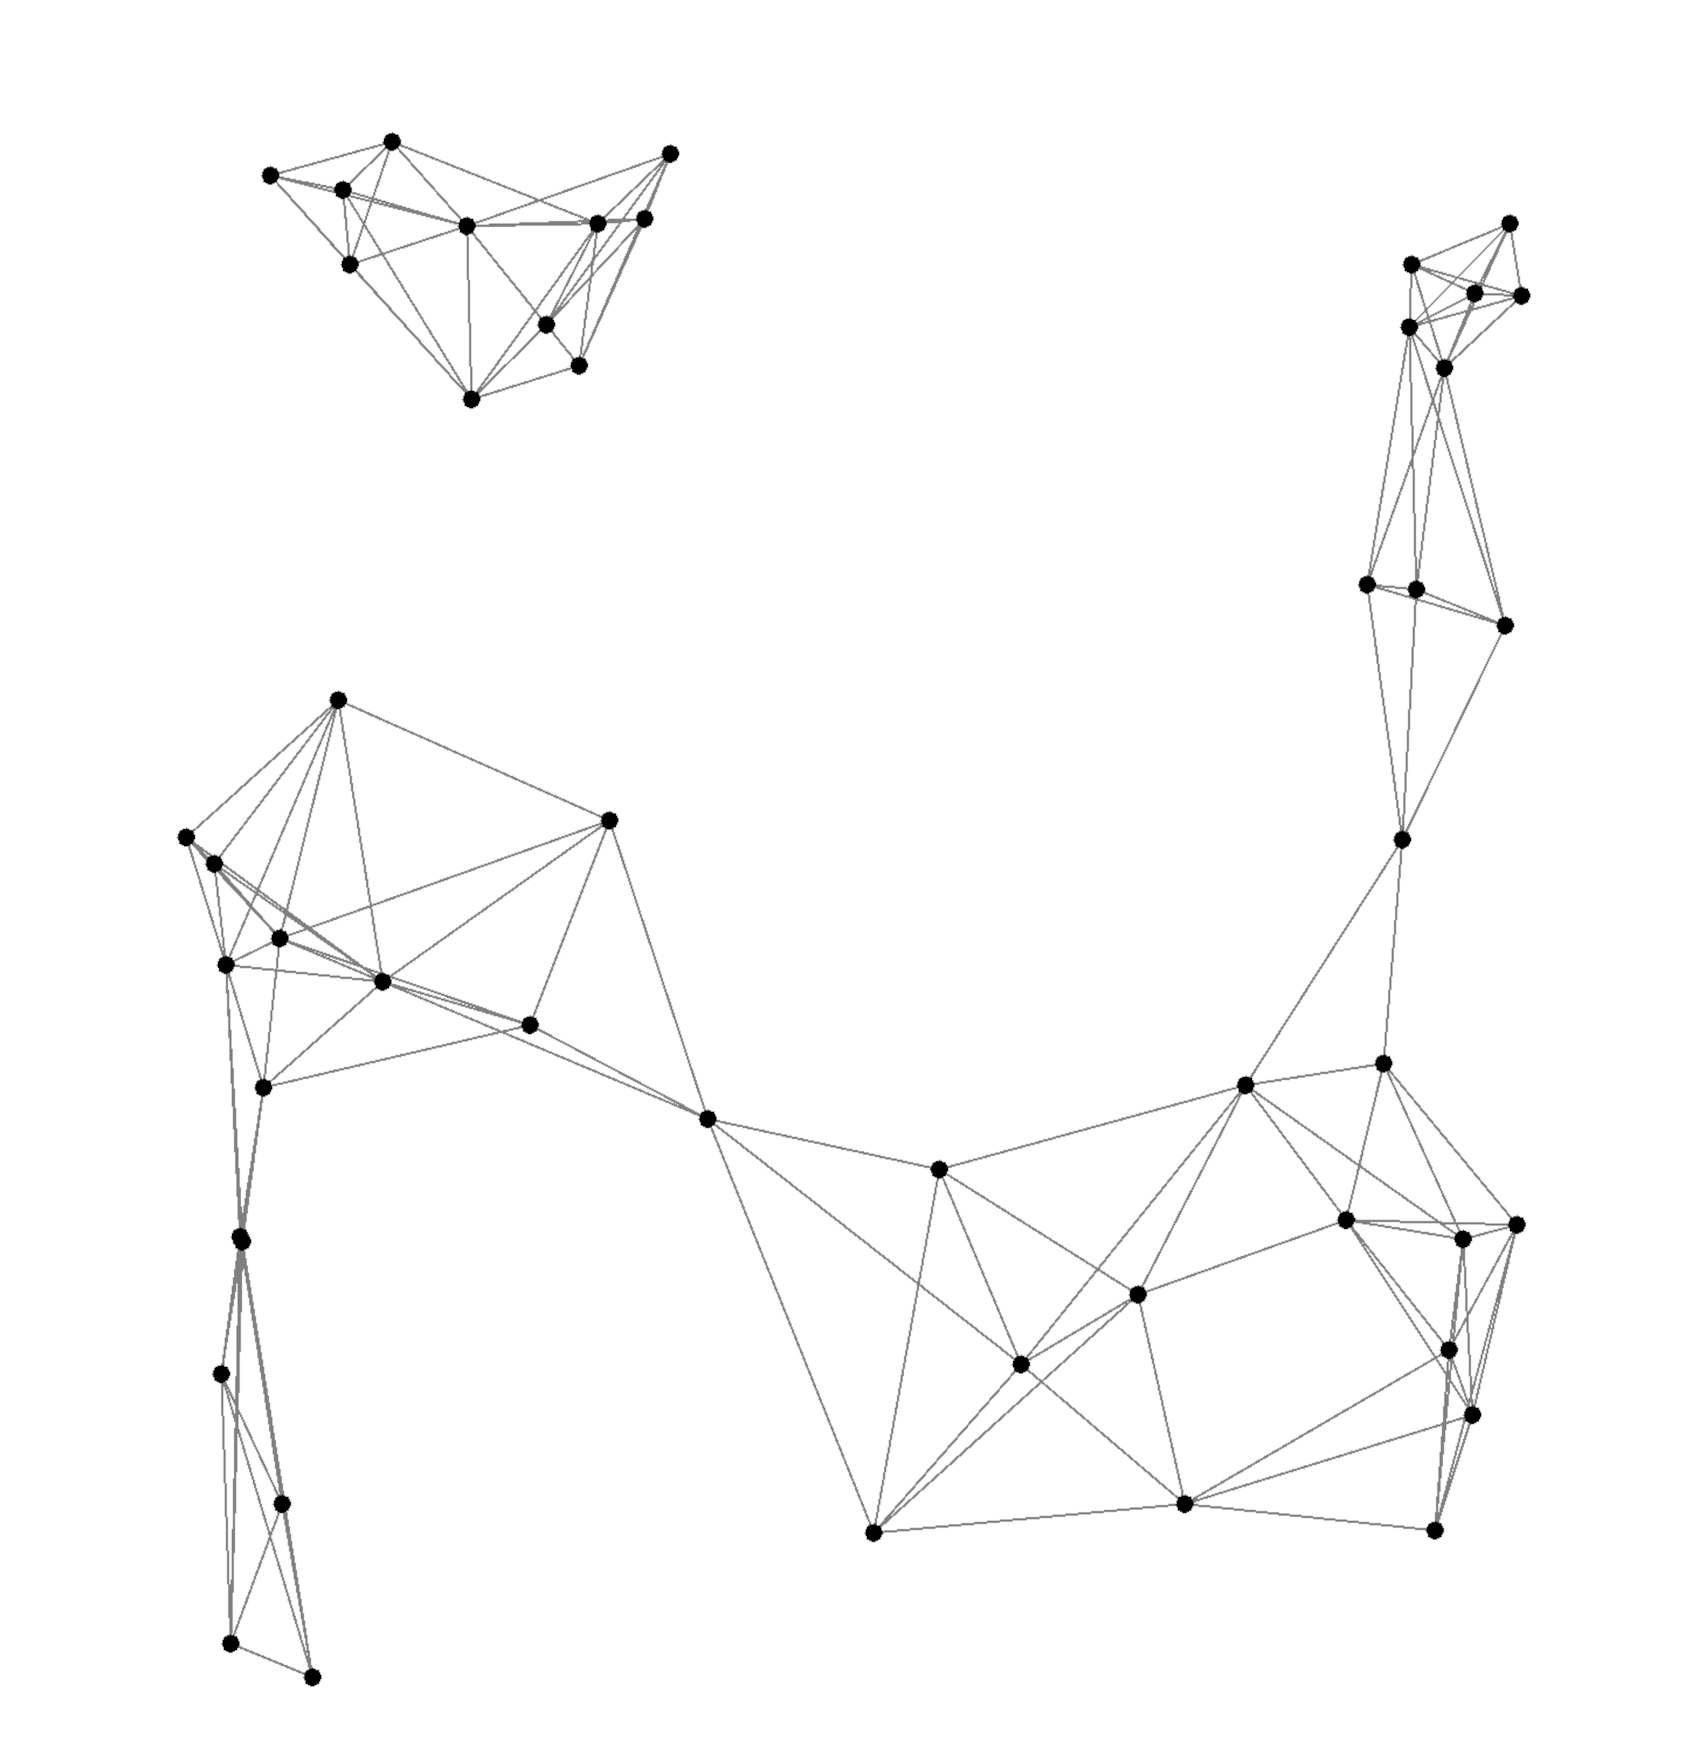
\includegraphics[width=\textwidth]{papers/coordination2023/imgs/4.png}}
        \caption{}
    \end{subfigure}
    \hfill
    \begin{subfigure}[b]{0.25\textwidth}
        \centering
        \fbox{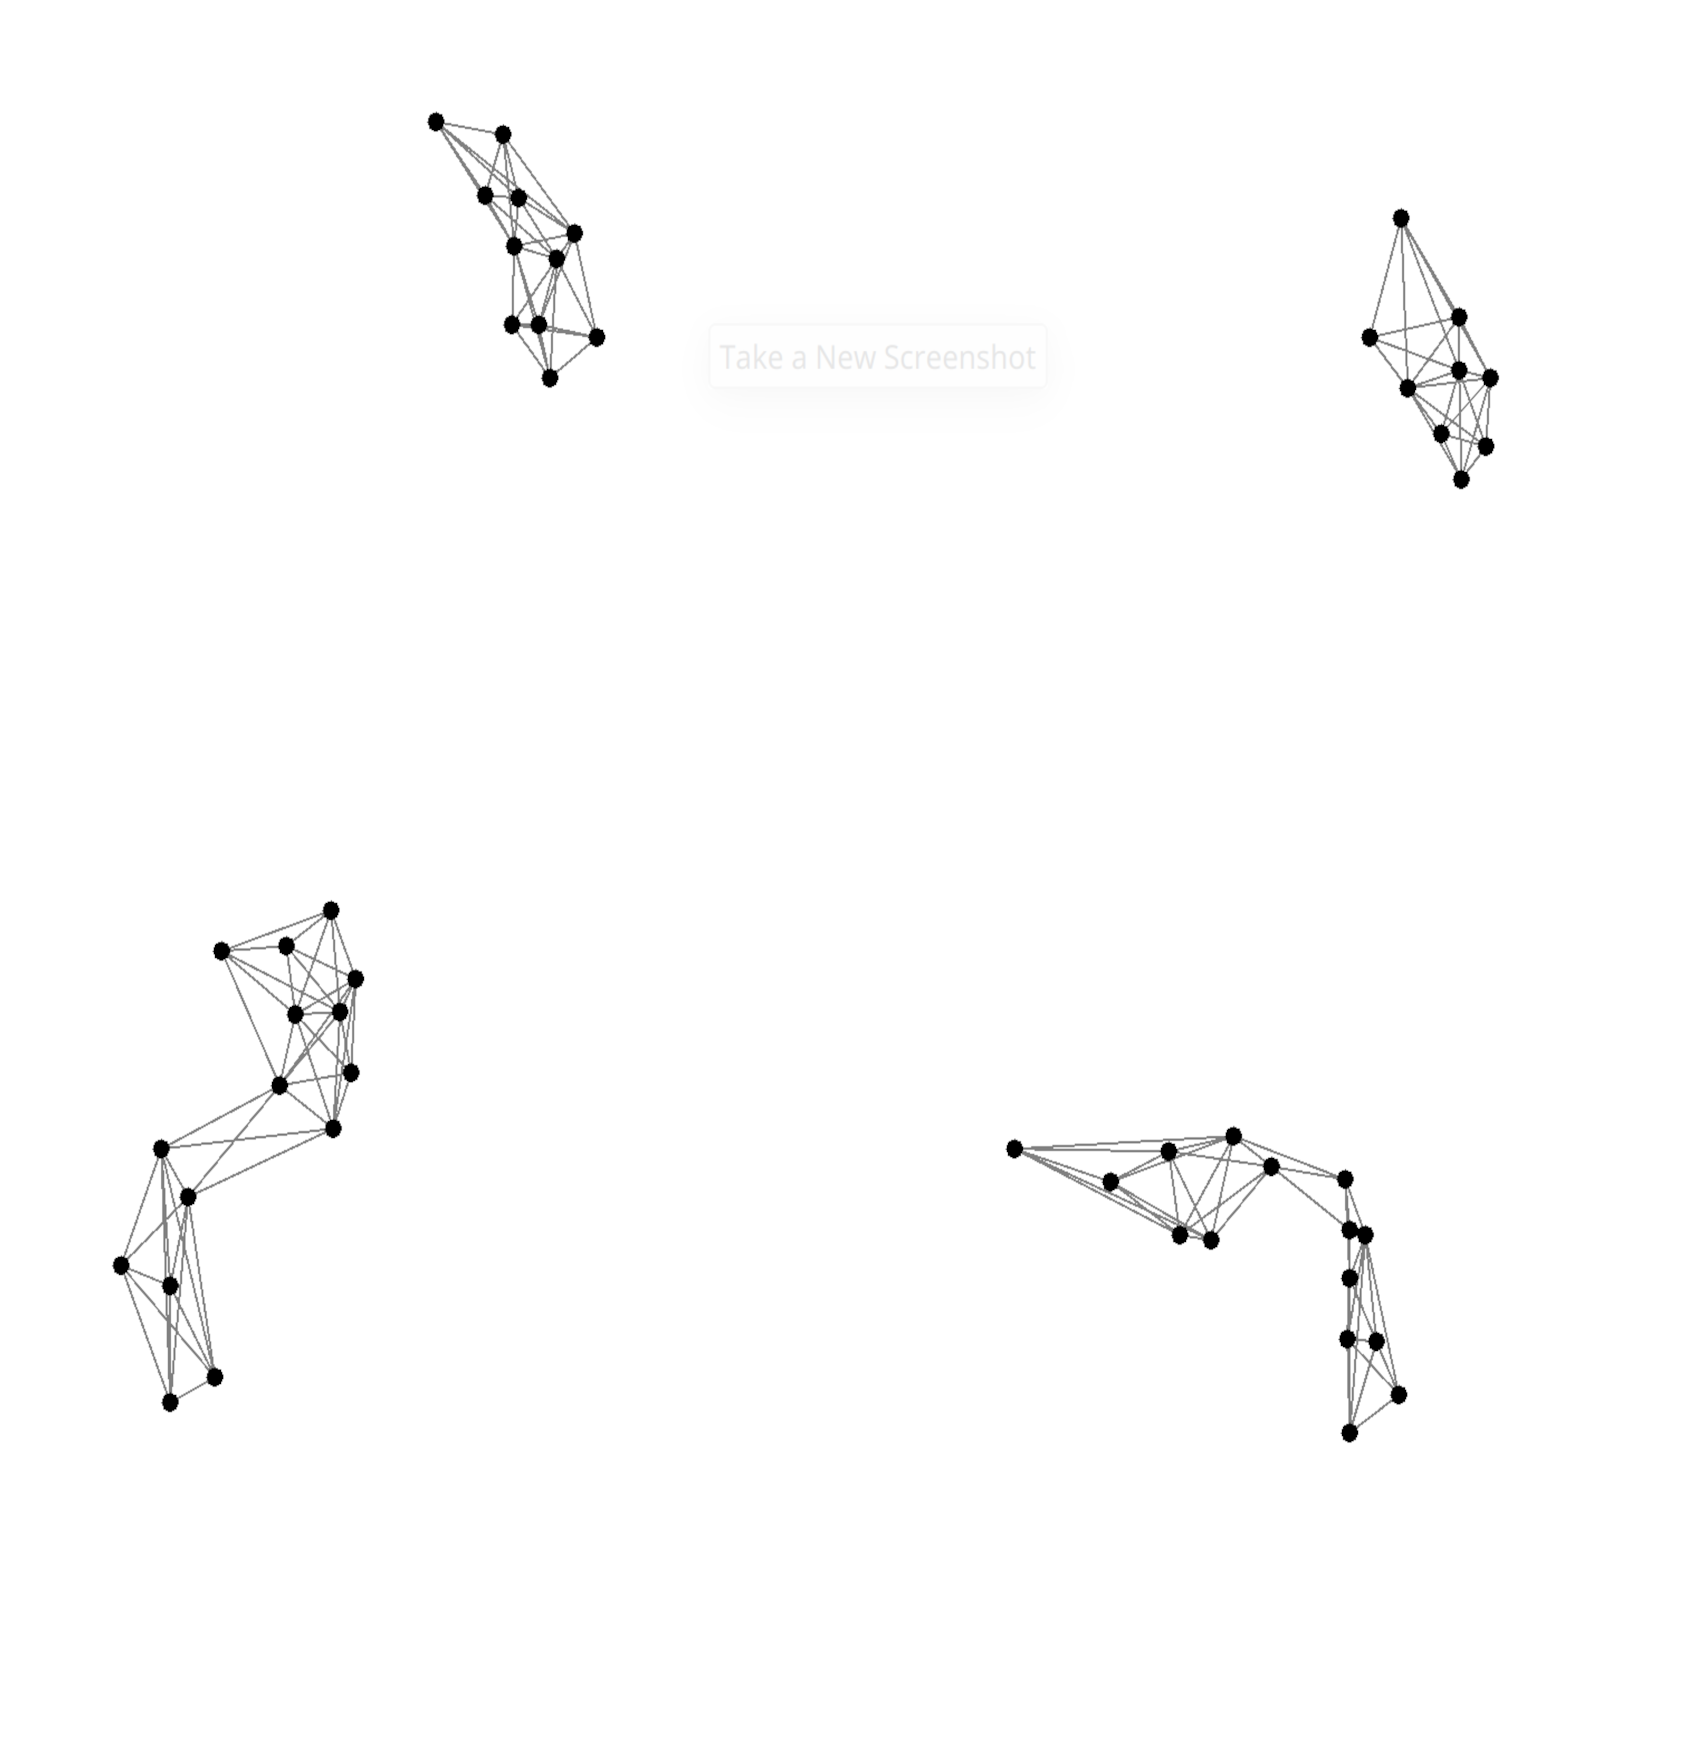
\includegraphics[width=\textwidth]{papers/coordination2023/imgs/7.png}}
        \caption{}
    \end{subfigure}
    \par
    \begin{subfigure}[b]{0.25\textwidth}
        \centering
        \fbox{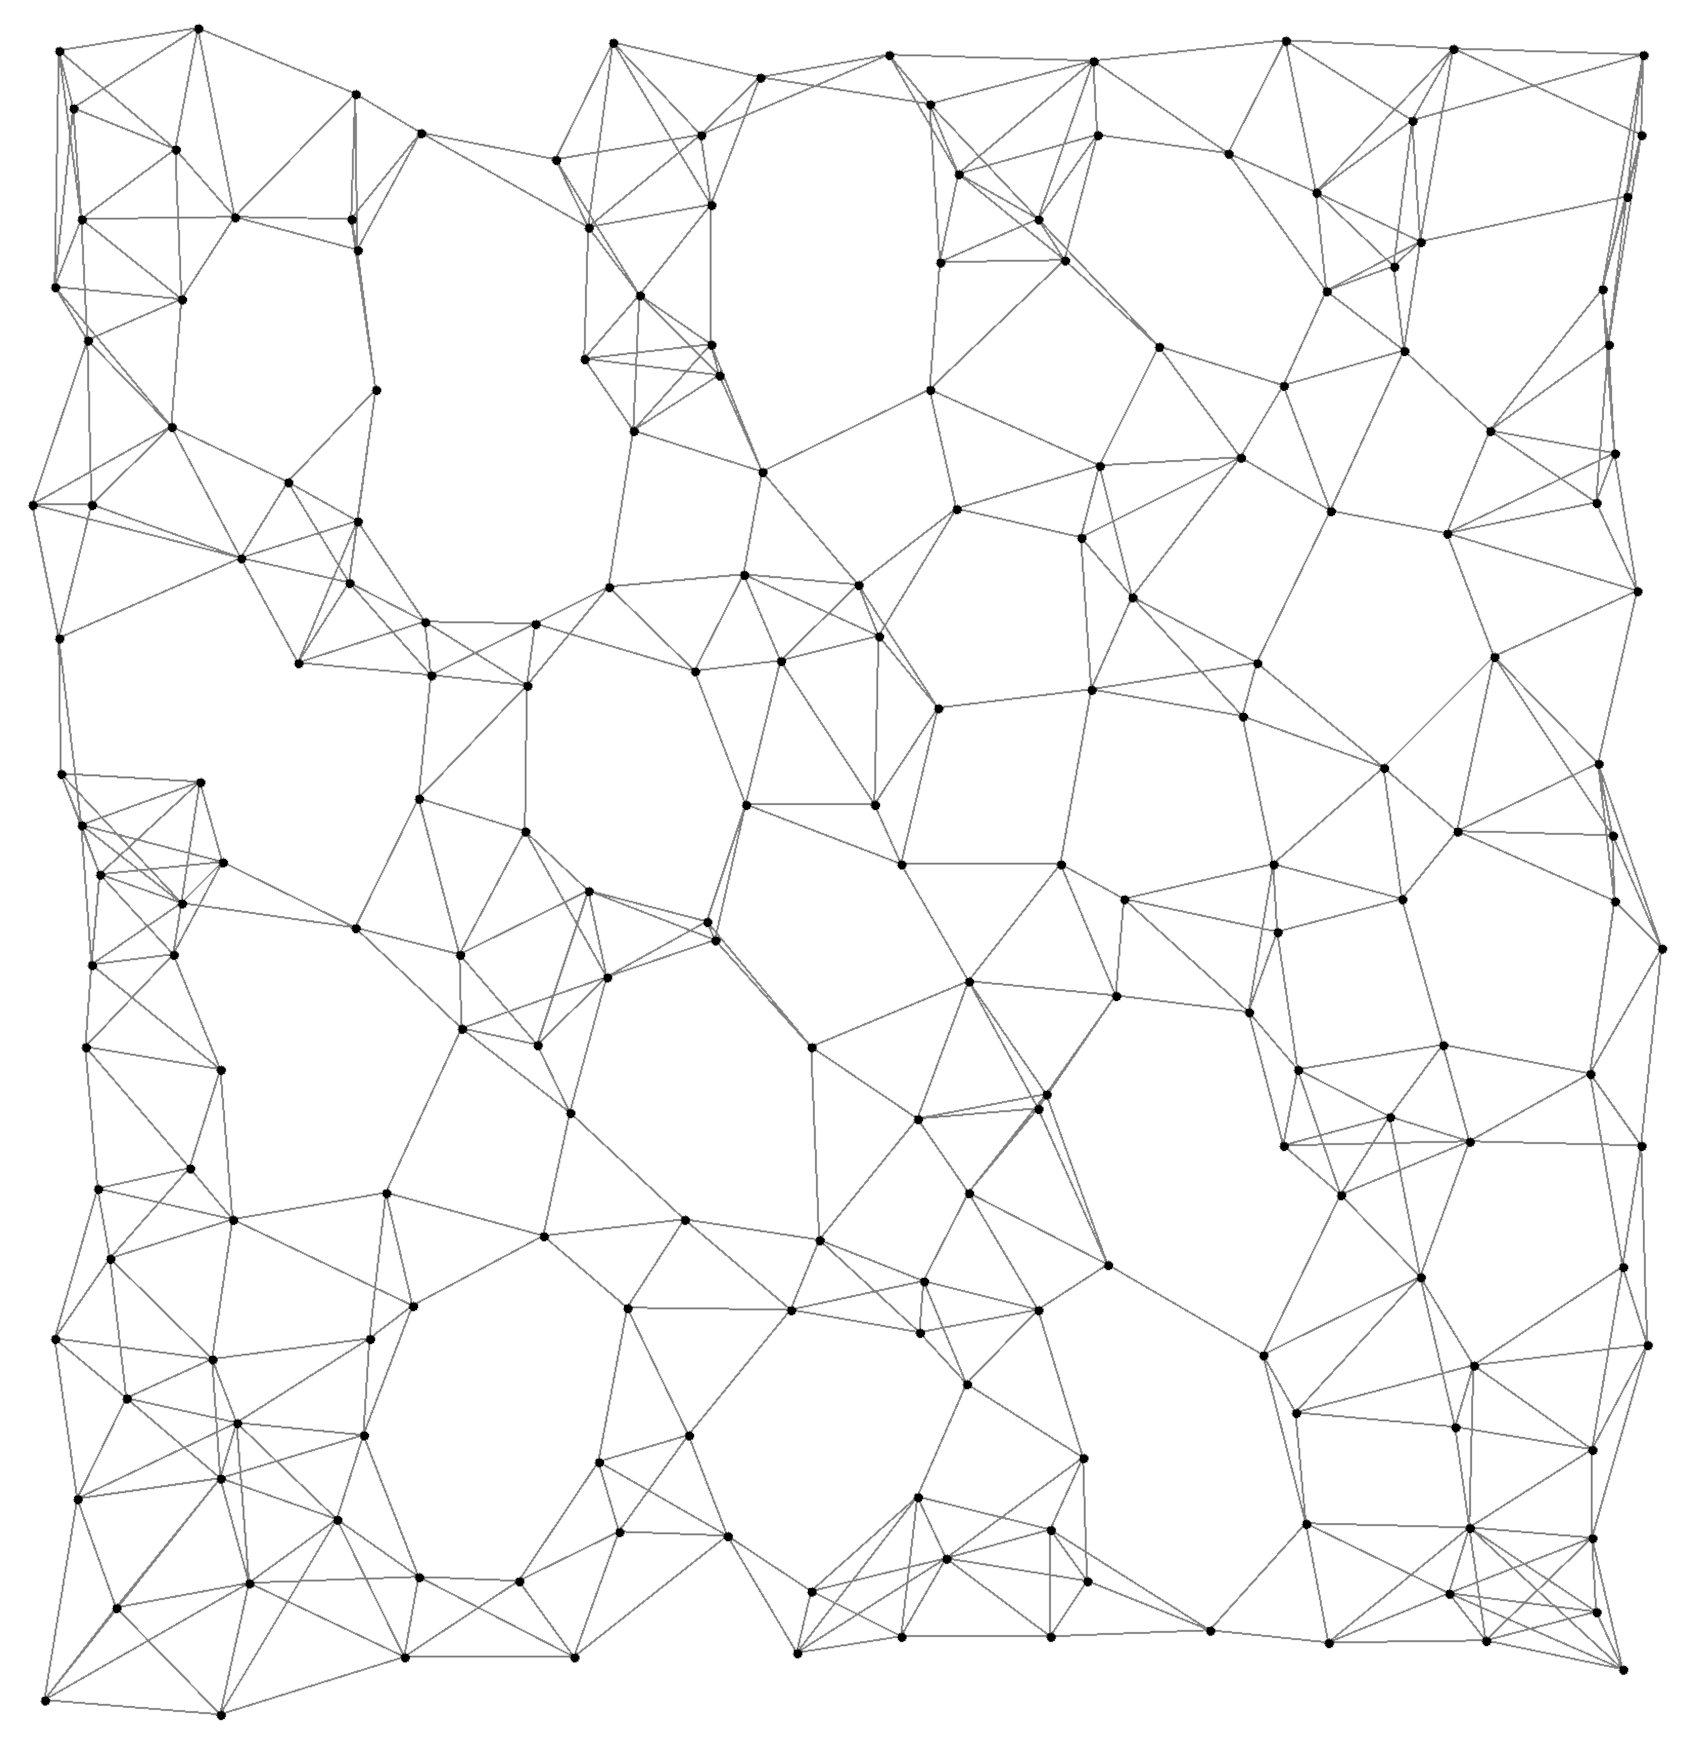
\includegraphics[width=\textwidth]{papers/coordination2023/imgs/1-large.png}}
        \caption{}
    \end{subfigure}
    \hfill
    \begin{subfigure}[b]{0.25\textwidth}
        \centering
        \fbox{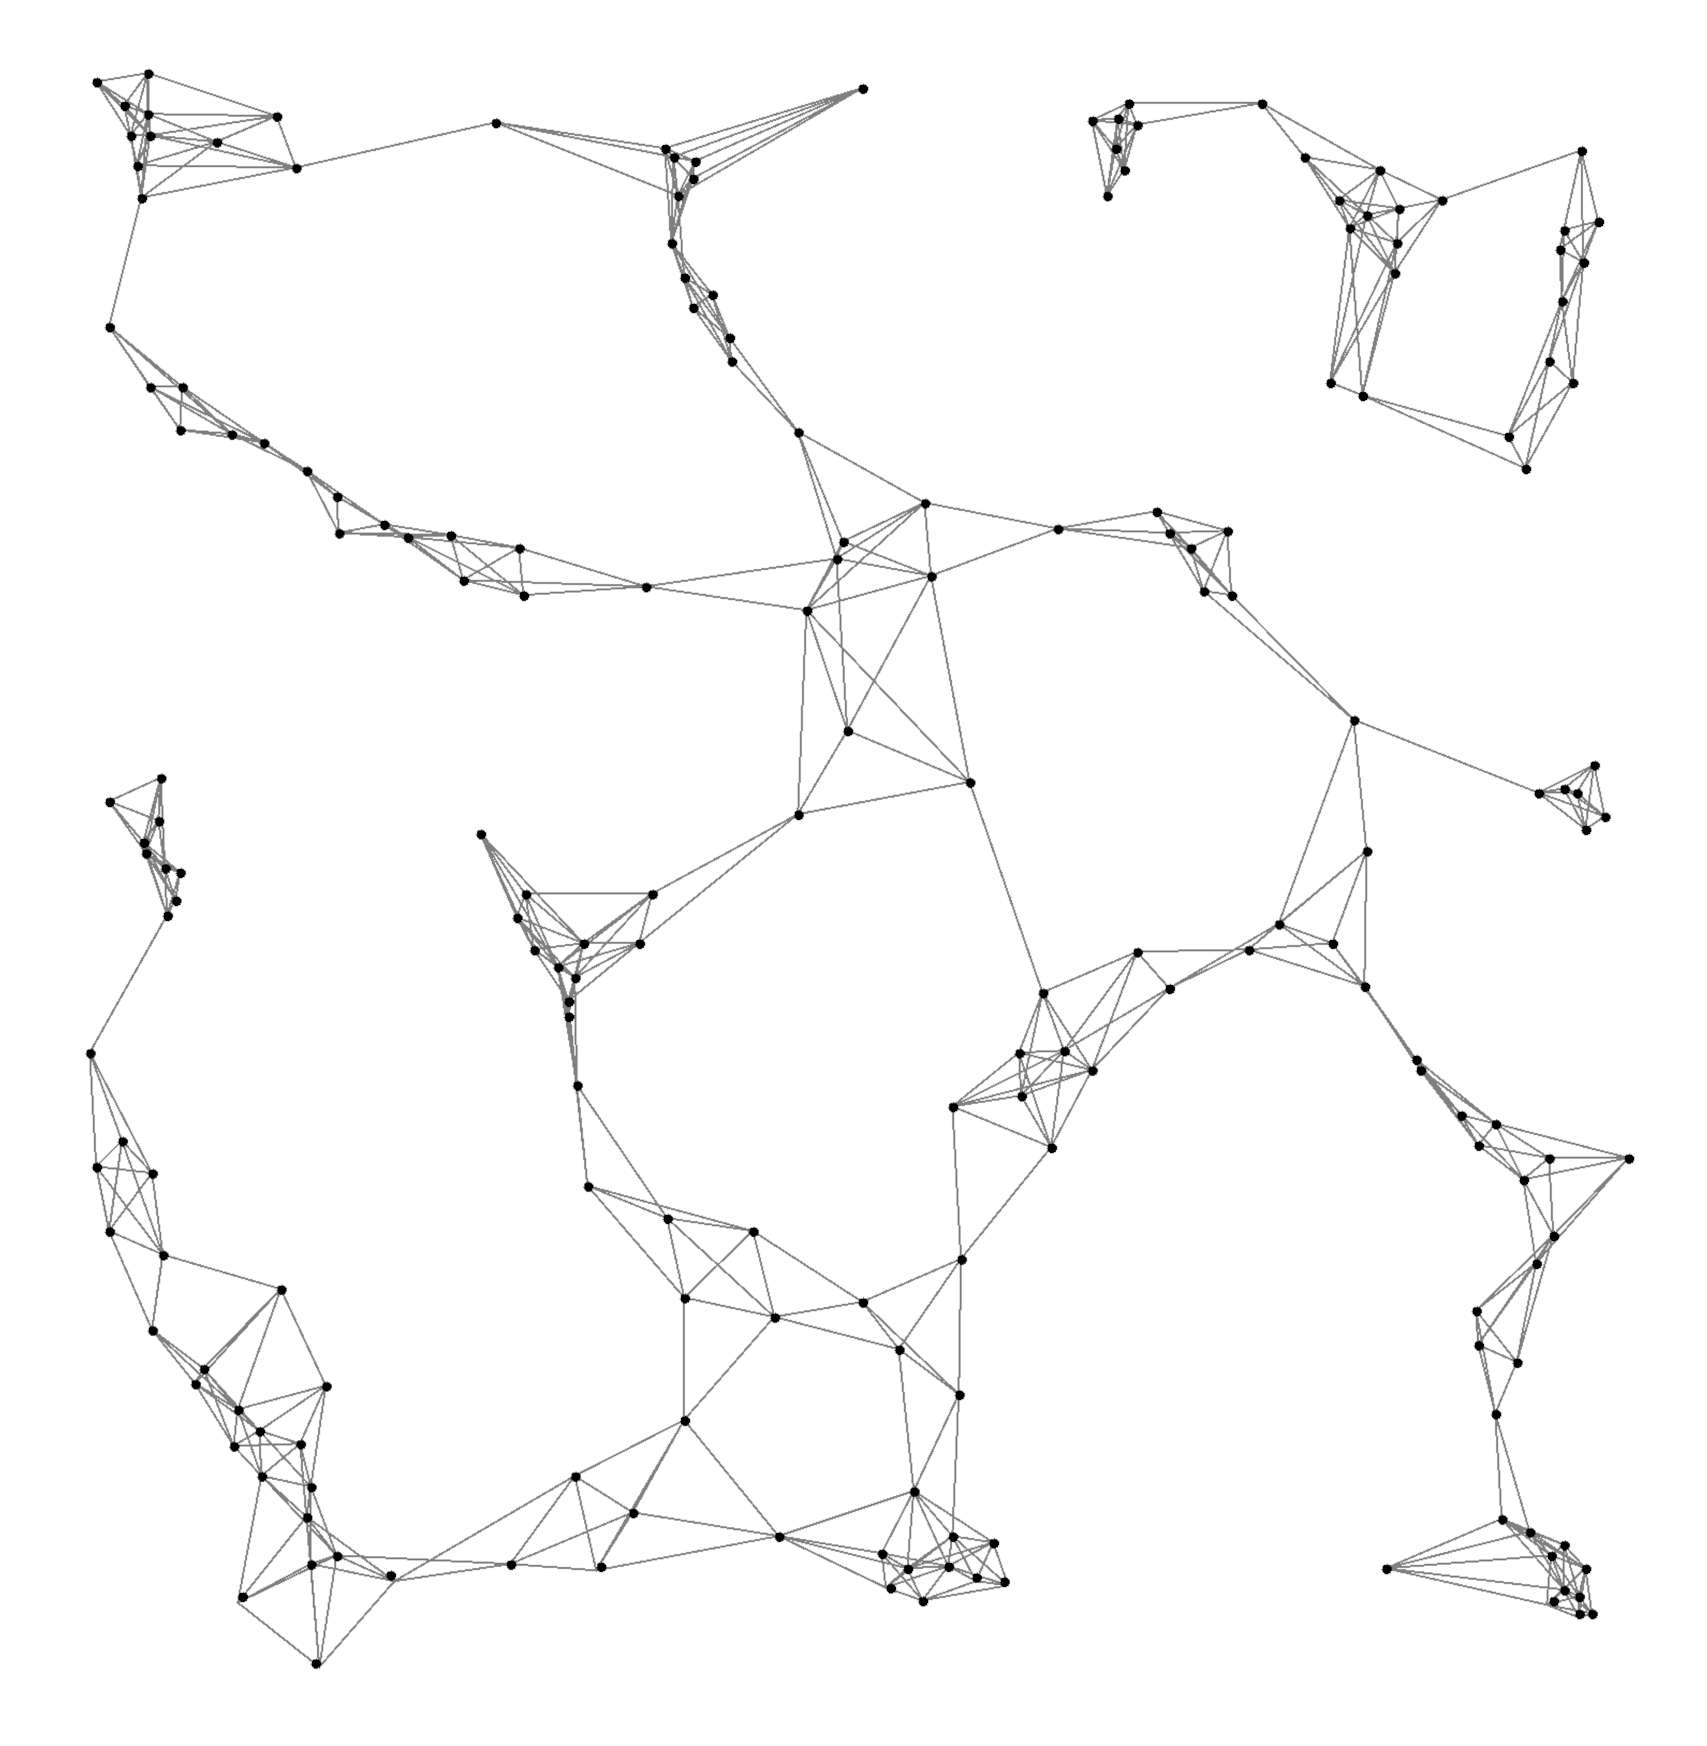
\includegraphics[width=\textwidth]{papers/coordination2023/imgs/3-large.png}}
        \caption{}
        \label{coordination2023:fig:sim2}
    \end{subfigure}
    \hfill
    \begin{subfigure}[b]{0.25\textwidth}
        \centering
        \fbox{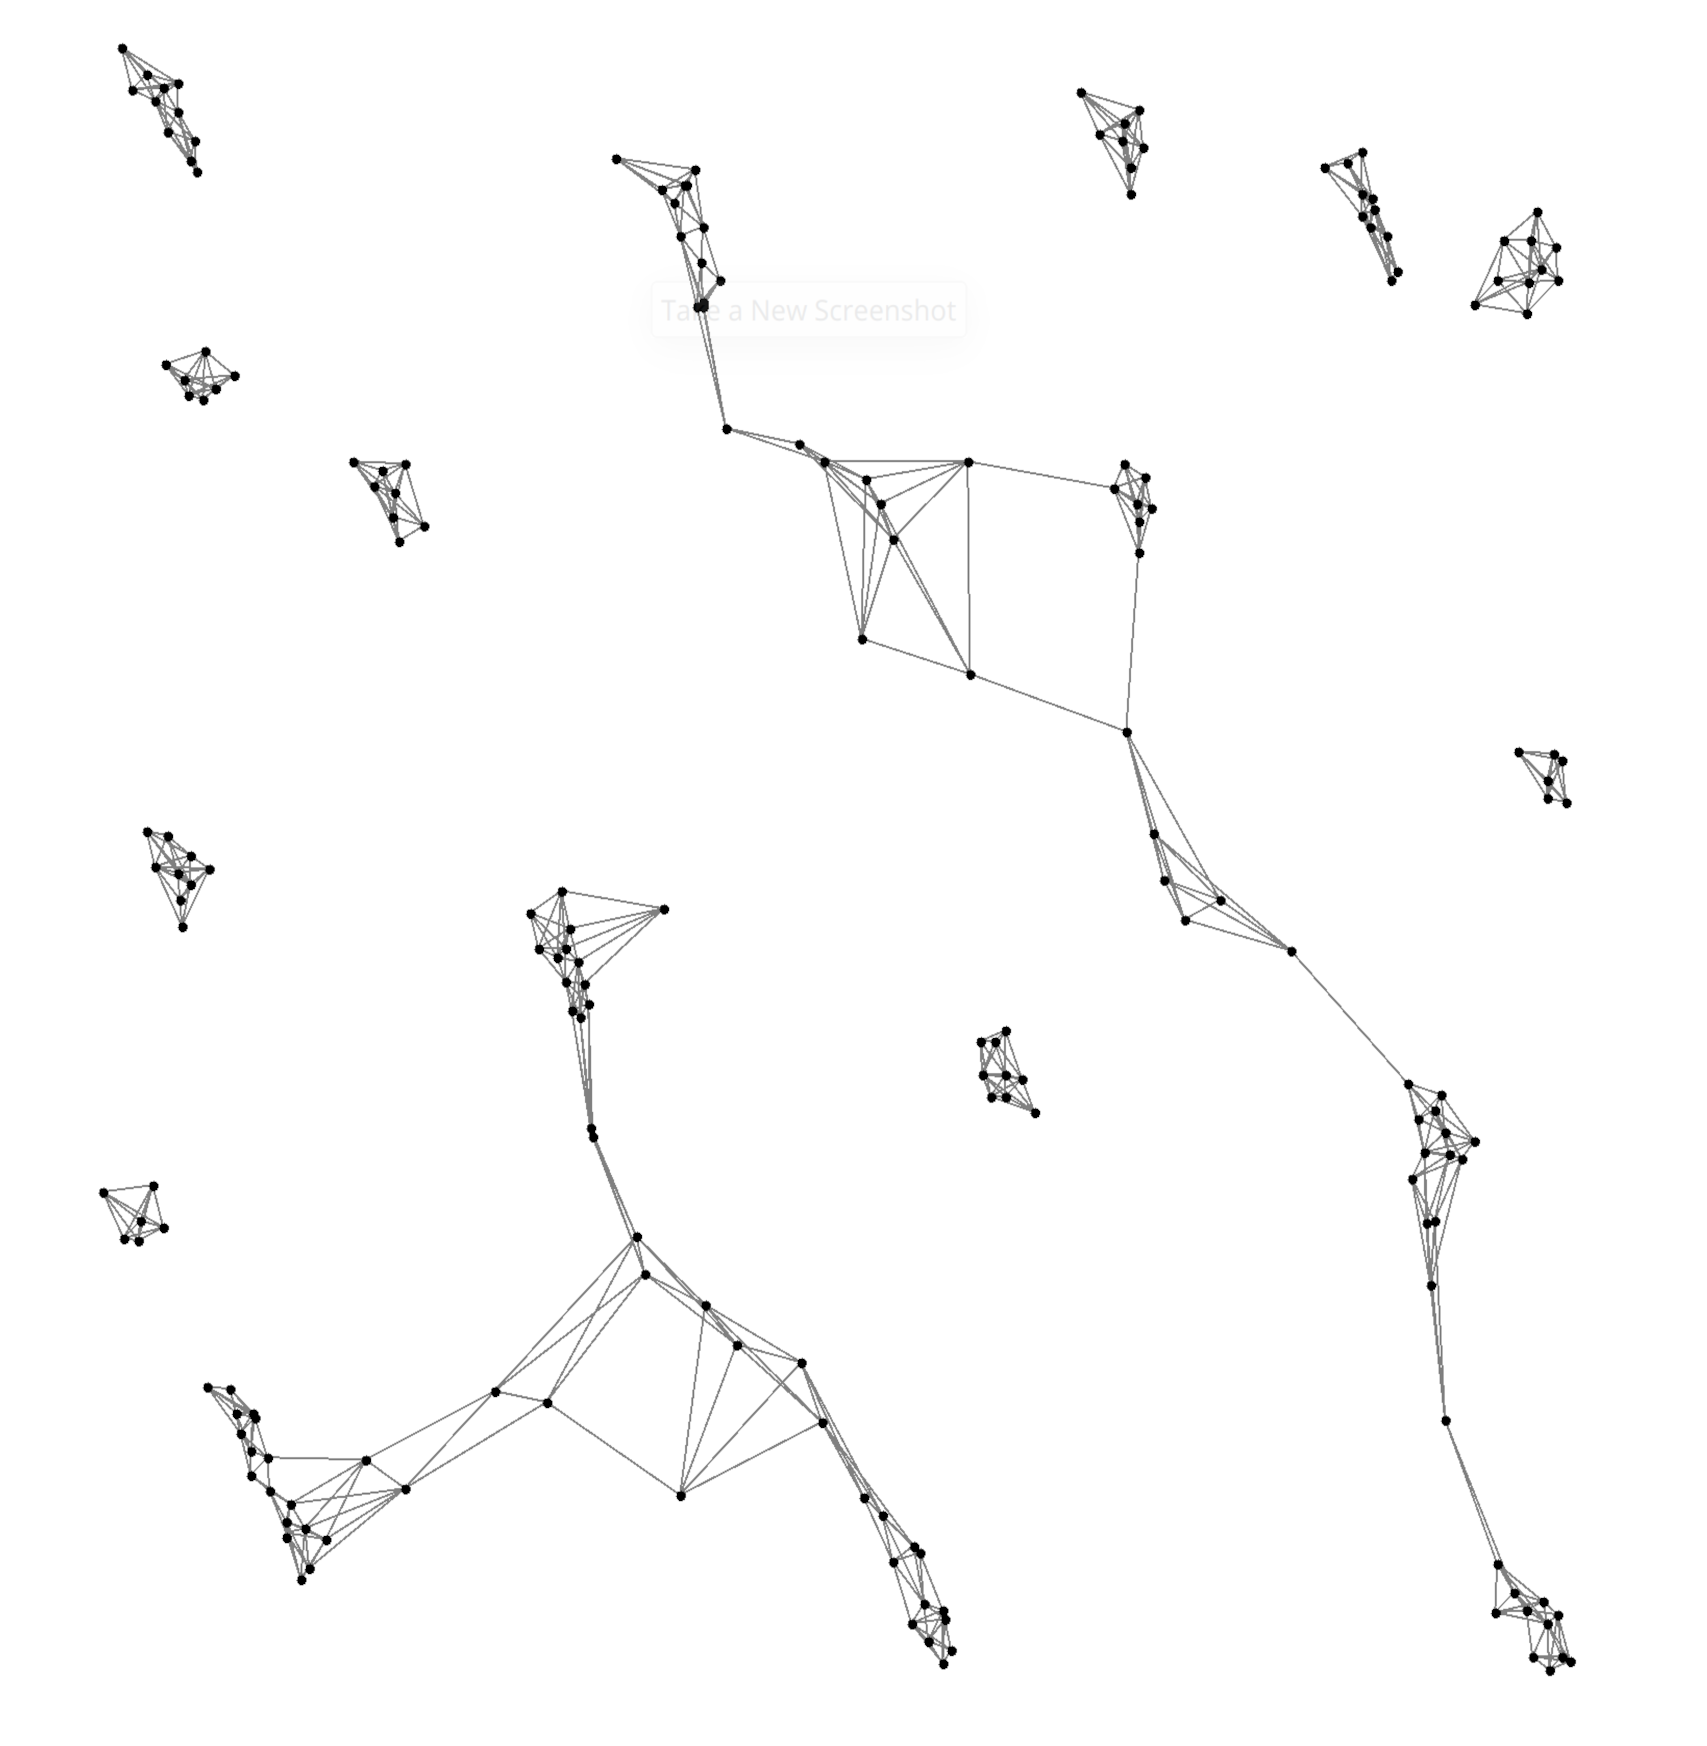
\includegraphics[width=\textwidth]{papers/coordination2023/imgs/4-large.png}}
        \caption{}
        \label{coordination2023:fig:sim3}
    \end{subfigure}
\caption[Snapshots of the learned policy in \scarlib{}]{Snapshots of the learned policy, the time flow is from left to right. 
In the first row, there are 50 agents, whereas in the second row, there are 200 agents.
In the last step of the simulation, the agents converged to a distance of approximately $\delta$.}
\label{coordination2023:fig:simulation-snapshots}
\end{figure*}

\begin{figure*}[h!]
    \centering
    \begin{subfigure}[b]{0.32\textwidth}
        \centering
        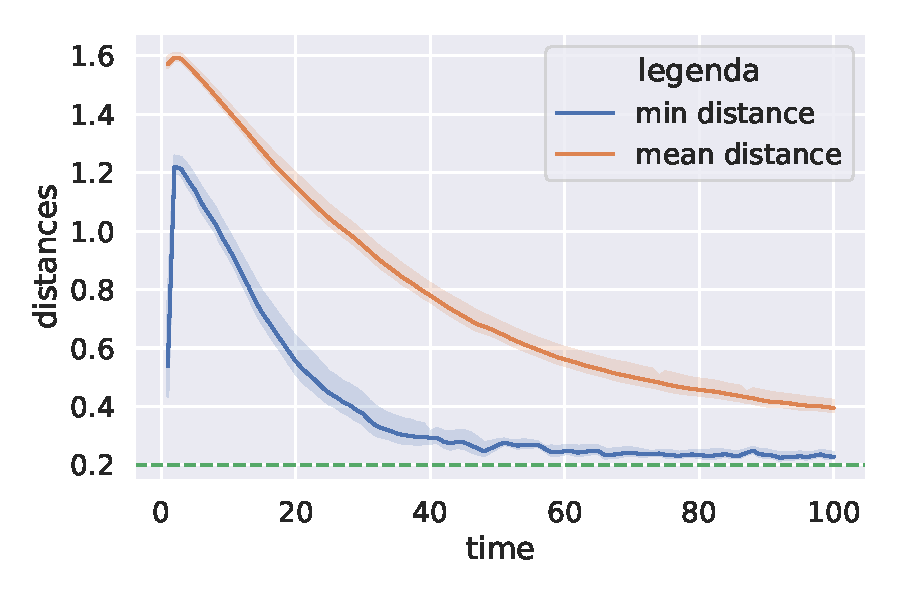
\includegraphics[width=\textwidth]{papers/coordination2023/imgs/data-50.pdf}
        \caption{50 agents}
    \end{subfigure}
    \hfill
    \begin{subfigure}[b]{0.32\textwidth}
        \centering
        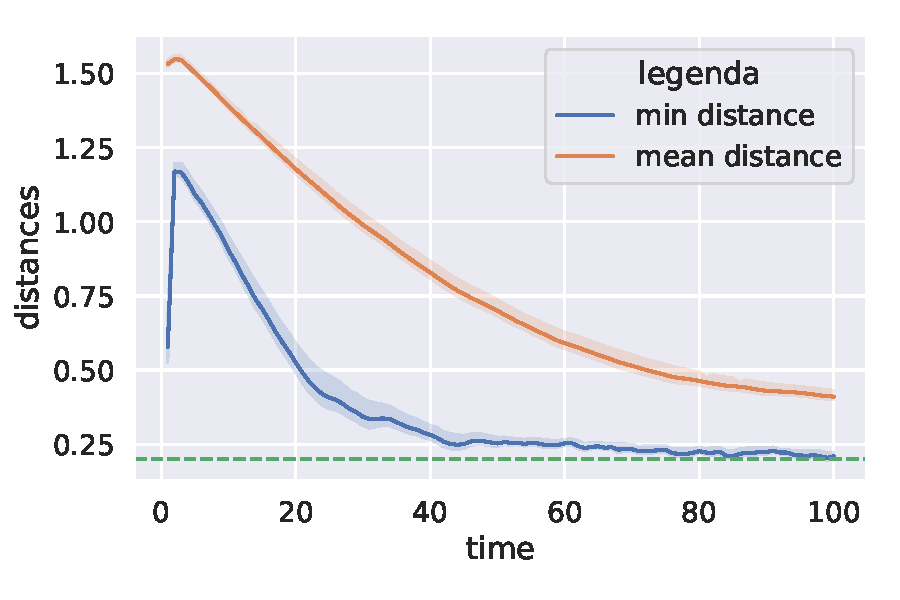
\includegraphics[width=\textwidth]{papers/coordination2023/imgs/data-100.pdf}
        \caption{100 agents}
    \end{subfigure}
    \hfill
    \begin{subfigure}[b]{0.32\textwidth}
        \centering
        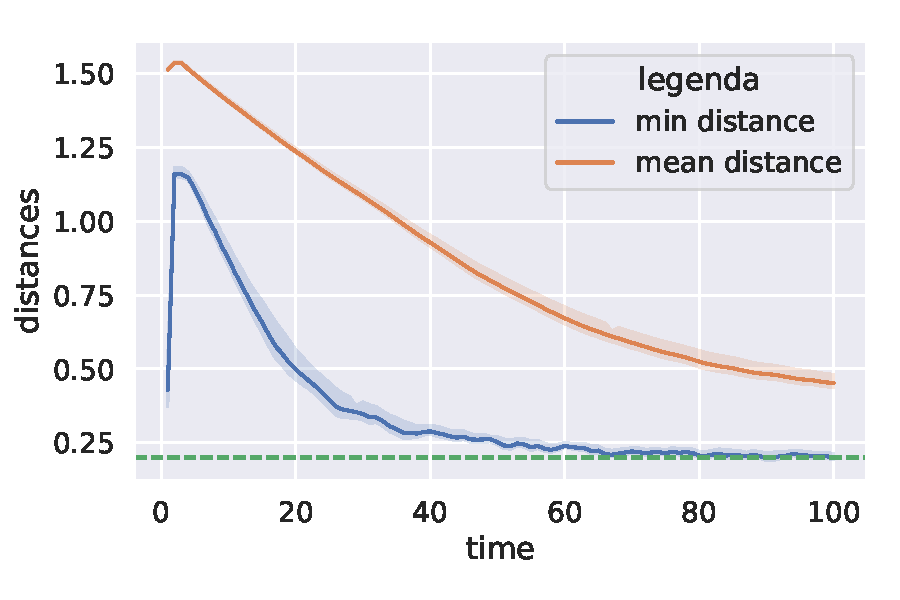
\includegraphics[width=\textwidth]{papers/coordination2023/imgs/data-200.pdf}
        \caption{200 agents}
    \end{subfigure}
\caption[The performance of the learned policy in \scarlib{}]{The performance of the learned policy. 
The y-axis represents the distance between the agents.
The x-axis represents the time.
The green line is equal to $\delta$.
In the charts, as the number of agents varies, the performance of the learned policy is similar.
Moreover, the minimum (blue line) distance between the agents is always greater than $\delta$.
The average distance (orange line) stays close to 2 * $\delta$ (after convergence).
}
\label{coordination2023:fig:test}
\end{figure*}

%\paragraph{Results}
%Here you should show the result of the cleaning robot experiment
\section{Related work}\label{coordination2023:sec:related}
MARL has gained significant interest in the past decade, 
 leading to the development of several frameworks 
 for use in both research and industry communities. 
Here, we highlight current state-of-the-art solutions 
 for MARL problems and compare 
 them to the tools presented in this work.
\subsection{Many Agent simulators:}   
Unlike supervised learning, 
 where a large dataset is required to improve neural network performance, 
 in RL, algorithms require a simulator to gain experience. 
One such comprehensive solution for MARL is PettingZoo~\cite{NEURIPS2021_7ed2d345}, 
 which provides both competitive and cooperative settings 
 for simulations with multiple agents. 
%
Another option for many-agent scenarios is NeuralMMO~\cite{https://doi.org/10.48550/arxiv.1903.00784}, 
 a GPU-optimized simulator for MMO-like games 
 that is designed to handle large-scale simulations of thousands of agents.
% 
Vectorized Multi-agent Simulator~\cite{bettini2022vmas} is another promising solution, 
 as it is optimized for collective tasks through GPU computation, 
 and it can be extended with additional environments.
%
While \scarlib is not directly linked to any simulator, 
 its main abstraction can be potentially linked 
 to both JVM-based simulators and gym-based Python environments. 
 Our choice of Alchemist was mainly due to its ability to express \ac{MAARL} settings easily, but potentially it can be used with any of the above-described solutions.
\subsection{Multi-Agent Deep RL libraries:}
since the importance of multi-agent settings several libraries have been developed in recent years. 
Ray~\cite{ray} is one of the most comprehensive frameworks, 
 originally designed for single-agent RL but 
 now integrated with basic concepts for MARL solutions thanks to MALib. 
It offers various MARL algorithms,
 supports different gym-like environments, 
 and is highly customizable through configuration files. 
%
PyMARL~\cite{samvelyan19smac} is one of the first solutions in Python for MARL, 
 though it is limited to specific algorithms (like VDN and QMIX), 
 and it is not generalizable. 
%
\scarlib{} is more similar to the first framework, 
 even though it is primarily designed for cooperative applications. 
%
However, since it was developed specifically for \ac{MAARL}, 
 it includes some abstractions and configurations that are not present in Ray, 
 such as the concept of a collective reward function and the configuration for CTDE. 
%
This reduces the time required to use \scarlib{} compared to Ray. 
 Additionally, \scarlib{} has a simple DSL that is easier to use than Ray's configuration system and is aided by the type system.

Finally, some innovative approaches aim to scale solutions to large populations of cooperative agents, such as mean-field RL. However, only a few implementations currently exist, and they are not considered to be general-purpose. \scarlib{}, on the other hand, offers a practical, simple implementation that can be leveraged in \ac{MAARL} settings.

Overall, \ac{MAARL} is a high-level framework that reduces the effort required for developers and practitioners to define and implement \ac{MAARL} problems when compared to current state-of-the-art solutions.

\subsection{Many-Agent Proof of Concept:}
The above RL library solutions are mainly created for multi-agent systems, 
 so they generally do not scale well with large populations of agents. 
 Novel approaches aim to scale the solution to potentially infinite populations of cooperative agents. 
In particular, mean-field RL~\cite{meanfield} is probably one of the 
 most interesting solutions in this context, 
 as it abstracts over the entire agent population 
 by considering only the average response of the neighbourhood. 
%
Currently, however, only a few implementations 
 exist~\footnote{\url{https://github.com/mlii/mfrl}} and they are not considered to be general-purpose. 
 \scarlib{} instead is practical and already provides a simple implementation that can be leveraged in \ac{MAARL} settings. 
\section{Final Remarks}\label{coordination2023:conclusion}
In this chapter, we presented \scarlib{}: 
 a collaborative many-agent deep reinforcement learning framework that integrates the functionalities of \scafi{} and Alchemist.
%
 The framework enables the definition of simulations of large-scale distributed scenarios 
 and the creation of complex scenarios with ease through its exposed DSL. 
% 
With \scarlib{}, developers can effectively and efficiently simulate and experiment with different reinforcement learning algorithms, 
 thereby providing a valuable tool for the advancement of coordination and multi-agent systems research.
This tool is essential in the view presented in this thesis: 
 the development of Cyber-Physical Swarms applications need both a foundational theory and a practical tool to test and validate the theory.
%
%
% ---- Bibliography ----
%
% BibTeX users should specify bibliography style 'splncs04'.
% References will then be sorted and formatted in the correct style.
%
%\printbibliography